\documentclass{article}
\usepackage{helvet}
\usepackage{geometry}
\usepackage{graphicx}
\usepackage{fancyhdr}
\usepackage{sectsty}
\usepackage{hyperref}
\usepackage{blindtext}
\usepackage{amsmath}
\usepackage{siunitx}
\usepackage{listings}
\usepackage{hyperref}
\usepackage[spanish]{babel}
\renewcommand{\familydefault}{\sfdefault}
\setlength\headheight{43pt} 
\usepackage[x11names]{xcolor}
\usepackage{array}
\subsectionfont{\color[HTML]{DDCB77}}
\sectionfont{\color[HTML]{2F6165}}
\hypersetup{
    colorlinks=true,
    linkcolor=black,
    filecolor=magenta,      
    urlcolor=black,
    pdftitle={Instructivo},
    pdfpagemode=FullScreen,
    citecolor=black
    }
\geometry{a4paper, bottom=3cm}
\lstset{
  basicstyle=\ttfamily,
  columns=fullflexible,
  frame=single,
  breaklines=true,
  postbreak=\mbox{\textcolor{blue}{$\hookrightarrow$}\space},
}

% PORTADA
\renewcommand{\maketitle}{
    \begin{titlepage}
            \begin{center}
                
\includegraphics[width=1\textwidth]{img/FCEFyN-Duotono_tagline.png}
            
            \vspace*{1cm}
                
            \Huge
            \textbf{Informe de Actividad Nº1}
                
            \vspace{0.5cm}
            \LARGE
            Representación de Sistemas y Controladores

                
            
                
            \vfill
                
            \textbf{Facundo Nahuel Galvagno}

            \vspace{0.8cm}
                
            
                
            \Large
            Sistemas de Control II\\
            Universidad Nacional de Córdoba \\
            2024
        \end{center}
                
    \end{titlepage}
}

% PIE Y TOPE DE PAGINA
\pagestyle{fancy}
\fancyhf{}
\fancyhead[C]{
\includegraphics[width=7cm]{img/color_UNC-FCEFyN.png}}
\fancyfoot[R]{\thepage}
\fancyfoot[L]{\textit{Sistemas de Control II - Actividad Nº1}}
\renewcommand{\headrulewidth}{0.1pt}
\renewcommand{\footrulewidth}{0pt}

\begin{document}

\lstset{language=Matlab,%
    %basicstyle=\color{red},
    breaklines=true,%
    morekeywords={matlab2tikz},
    keywordstyle=\color{Blue4},%
    morekeywords=[2]{1}, keywordstyle=[2]{\color{black}},
    identifierstyle=\color{black},%
    stringstyle=\color{Magenta1},
    commentstyle=\color{Green4},%
    showstringspaces=false,%without this there will be a symbol in the places where there is a space
    numbers=left,%
    numberstyle={\tiny \color{black}},% size of the numbers
    numbersep=9pt, % this defines how far the numbers are from the text
    emph=[1]{for,end,break},emphstyle=[1]\color{red}, %some words to emphasise
    %emph=[2]{word1,word2}, emphstyle=[2]{style},    
}

\maketitle

\tableofcontents
\newpage

\section{Introducción}
\label{section:1}
En este documento se detalla el desarrollo de la primera actividad
práctica propuesta por el profesor Julían Pucheta. Para el procesamiento 
computacional se utilizó MATLAB R2018a. La primicia del trabajo es la de utilizar fundamentos
de control sobre sistemas reales sobre los cuales se realizaron mediciones para obtener parámetros y
controlarlos.

La metodología para la resolución de los problemas se basó en el 
código y la teoría provistos en los apuntes de clase.

\section{Desarrollo}
\label{section:2}
\subsection{Caso de estudio 1. Sistema de dos variables de estado}
\label{subsection:1}
Sea el sistema eléctrico de la Fig. 1-1, con las representaciones en variables de estado

\begin{figure}[!h]
  \centering
  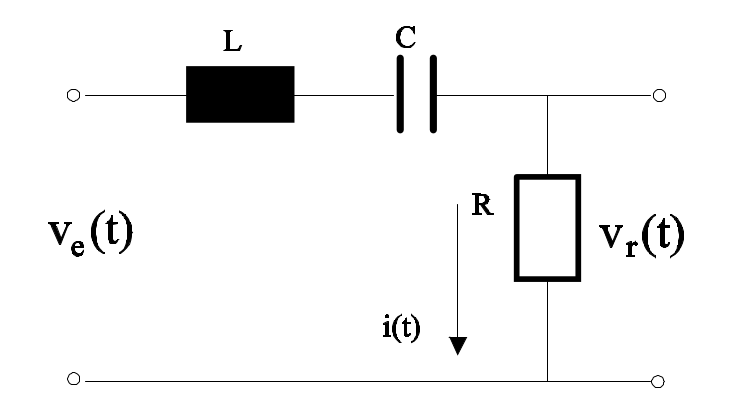
\includegraphics[width=0.35\textwidth]{img/1.png}
  \caption{Circuito RLC}
  \label{fig:1}
\end{figure}

$$\dot{X} = Ax(t)+Bu(t)$$
$$y=C*x(t)$$

donde las matrices contienen a los coeficientes del circuito,



\begin{equation}
  A = 
  \begin{bmatrix}
    -R/L & -1/L \\
    1/C & 0
  \end{bmatrix} 
  , B =
  \begin{bmatrix}
    1/L \\
    0
  \end{bmatrix} 
  , C = 
  \begin{bmatrix}
    R & 0
  \end{bmatrix} 
\end{equation}

\textbf{Ítem (1)} Asignar valores a $R=47\Omega$, $L=1\mu Hy$ y $C=100nF$. Obtener simulaciones que permitan
estudiar la dinámica del sistema, con una entrada de tensión escalón de 12V, 
que cada 1ms cambia de signo.

Para realizar la simulación del circuito RLC es indispensable conocer la dinámica del mismo.
Podemos obtener el valor de la dinámica más rápida y más lenta en base a los autovalores de la
matriz A, que son los polos de la función de transferencia del sistema.

\begin{lstlisting}[language=matlab]
R=47; L=1e-06; C=100e-09; %Parametros del circuito RLC
A1 = [-R/L -1/L; 1/C 0];
B1 = [1/L; 0];
C1 = [R 0];
C2 = [0 1]; 
D1 = [0];

eig_val = eig(A1)
\end{lstlisting}

Entonces, los autovalores de la matriz A son:

$$\lambda_1=\num{-4.57e7}, \lambda_2=\num{-2.13e5}$$

Para calcular el tiempo de integración y simulación, podemos encontrar el tiempo al que
corresponde el 95\% de la dinámica más rápida a partir de los polos de la función de
transferencia del sistema. Notar que el tiempo de
simulación debe ser el suficiente como para simular de correcta forma la entrada requerida, por lo tanto,
en lugar de observar la dinámica más lenta del sistema, simularemos el tiempo suficiente para que
la entrada de tensión conmute.


$$t_r = \frac{log(0.95)}{\lambda_1}$$
$$t_i \approx t_r/10 = \num{1e-10}$$
$$t_s = \num{5e-3}$$

\begin{lstlisting}[language=matlab]
%% Tiempo de integracion y simulacion
tr=log(0.95)/eig_val(1);

%Tomamos ti = 1e-10 (10 veces menor)
ti = 1e-10

%Tomamos ts = 5e-03 debido a que buscamos simular la 
%respuesta con una entrada que conmuta
ts = 5e-03 

N = ts/ti;
\end{lstlisting}

La cantidad de muestras de nuestro vector tiempo es:

$$N=\num{5e7}$$

Procedemos a simular el comportamiento del sistema mediante integración por Euler.

\begin{lstlisting}[language=matlab]
  %% Entrada y vector de tiempo
t = linspace (0, ts, N);
u = linspace (0, 0, N);

%Funciones i_c, v_c 

i_c=zeros(1,N);
v_c=zeros(1,N);


x = [0 0]'; %Cond. iniciales nulas
vin = 12;
ij = 0;

for ii=1:N-1
    ij=ij+ti;
    if (ij>=1e-3)
        ij=0;
        vin=vin*-1;
    end
    u(ii)=vin;
    xp=A1*x+B1*u(ii);
    x=x+xp*ti;
    Y=C1*x;
    y(ii+1)=Y(1);
    i_c(ii+1)=x(1);
    v_c(ii+1)=x(2);
end

figure('Name','1.1')
 subplot(3,1,1);plot(t,i_c);grid on; title('Corriente, I'); 
 subplot(3,1,2);plot(t,v_c);grid on; title('Tension del capacitor, V_c');
 subplot(3,1,3);plot(t,u);grid on; title('Tension de entrada, V_e');
 
\end{lstlisting}

\begin{figure}[!h]
  \centering
  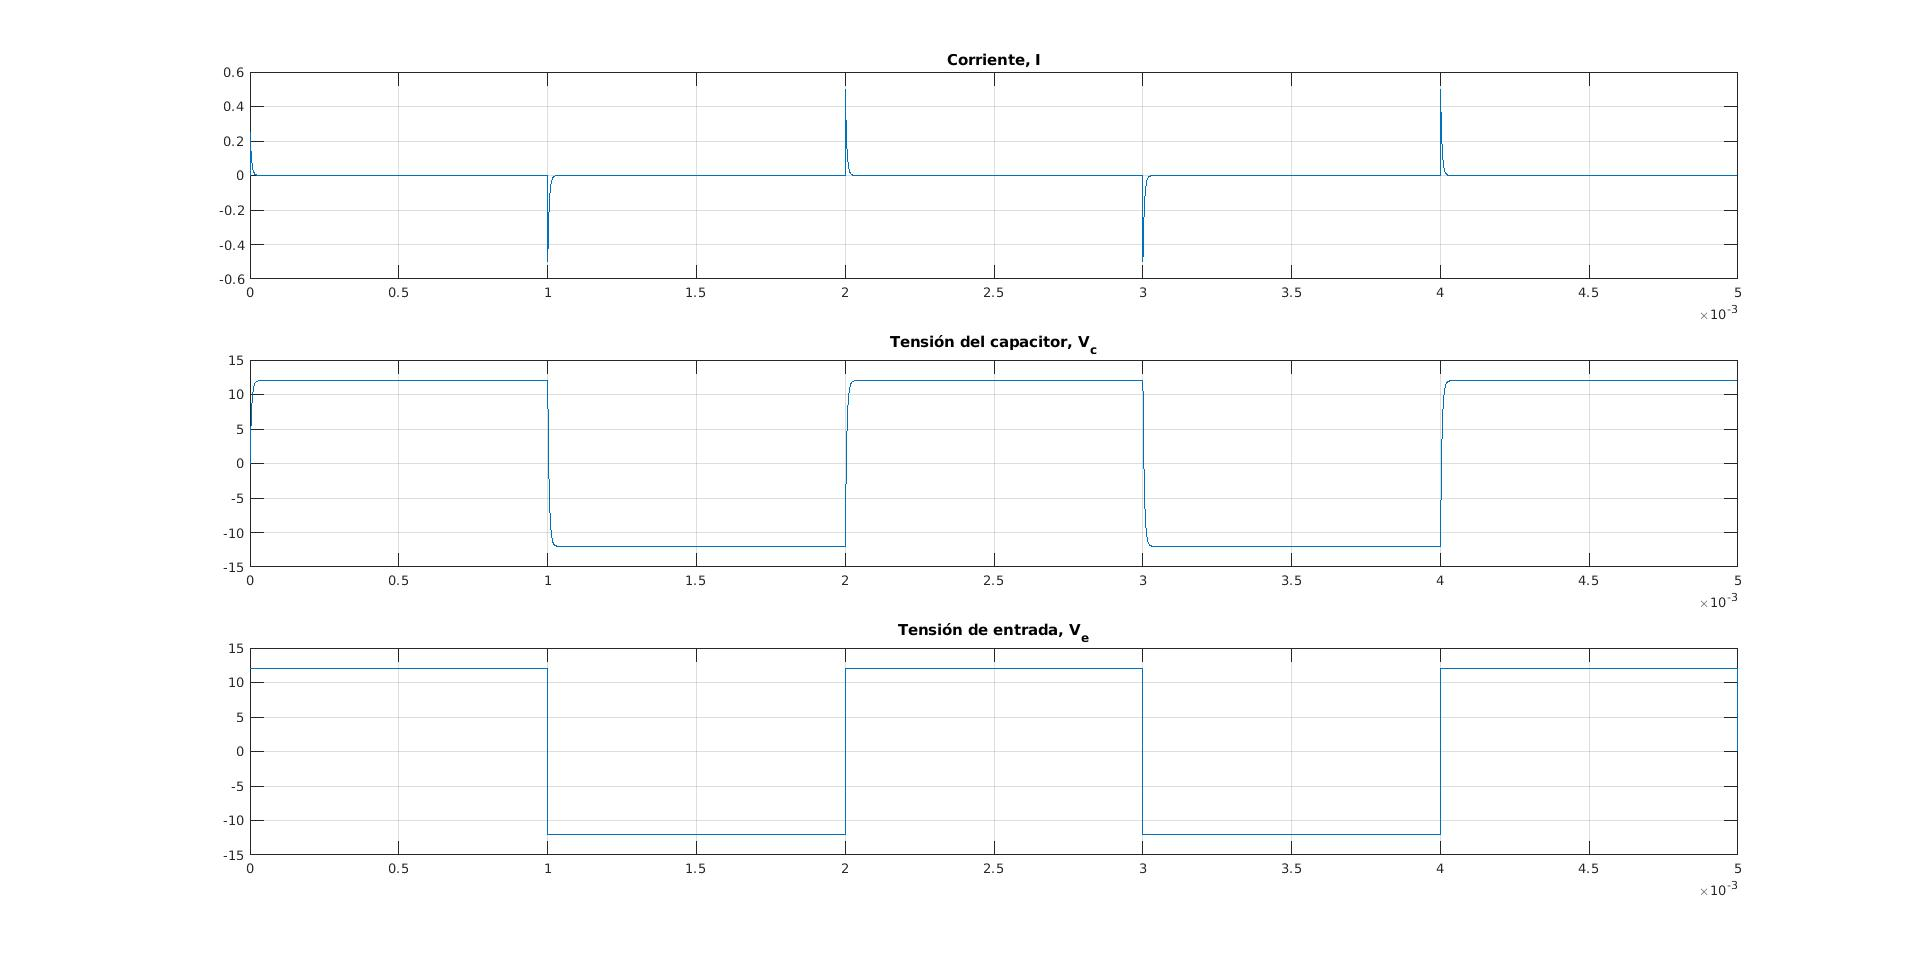
\includegraphics[width=1\textwidth]{img/rlc1-1.jpg}
  \caption{Respuesta del circuito RLC}
\end{figure}

\textbf{Ítem (2)} En el archivo \textit{Curvas\_Medidas\_RLC.xls} (datos en la hoja 1 y etiquetas en la hoja 2)
están las series de datos que sirven para deducir los valores de $R$, $L$ y $C$ del circuito. 
Emplear el método de la respuesta al escalón, tomando como salida la tensión en el capacitor.

\begin{lstlisting}[language=matlab]
datos = xlsread('Curvas_Medidas_RLC_2024.xlsx');
t = datos(:,1);
i = datos(:,2);
v_c = datos(:,3);

figure('Name', '1.2')
 subplot(2,1,1);plot(t,i);grid on; title('Corriente');
 subplot(2,1,2);plot(t,v_c);grid on; title('Tension en el capacitor, V_c1');

\end{lstlisting}

\begin{figure}[!h]
  \centering
  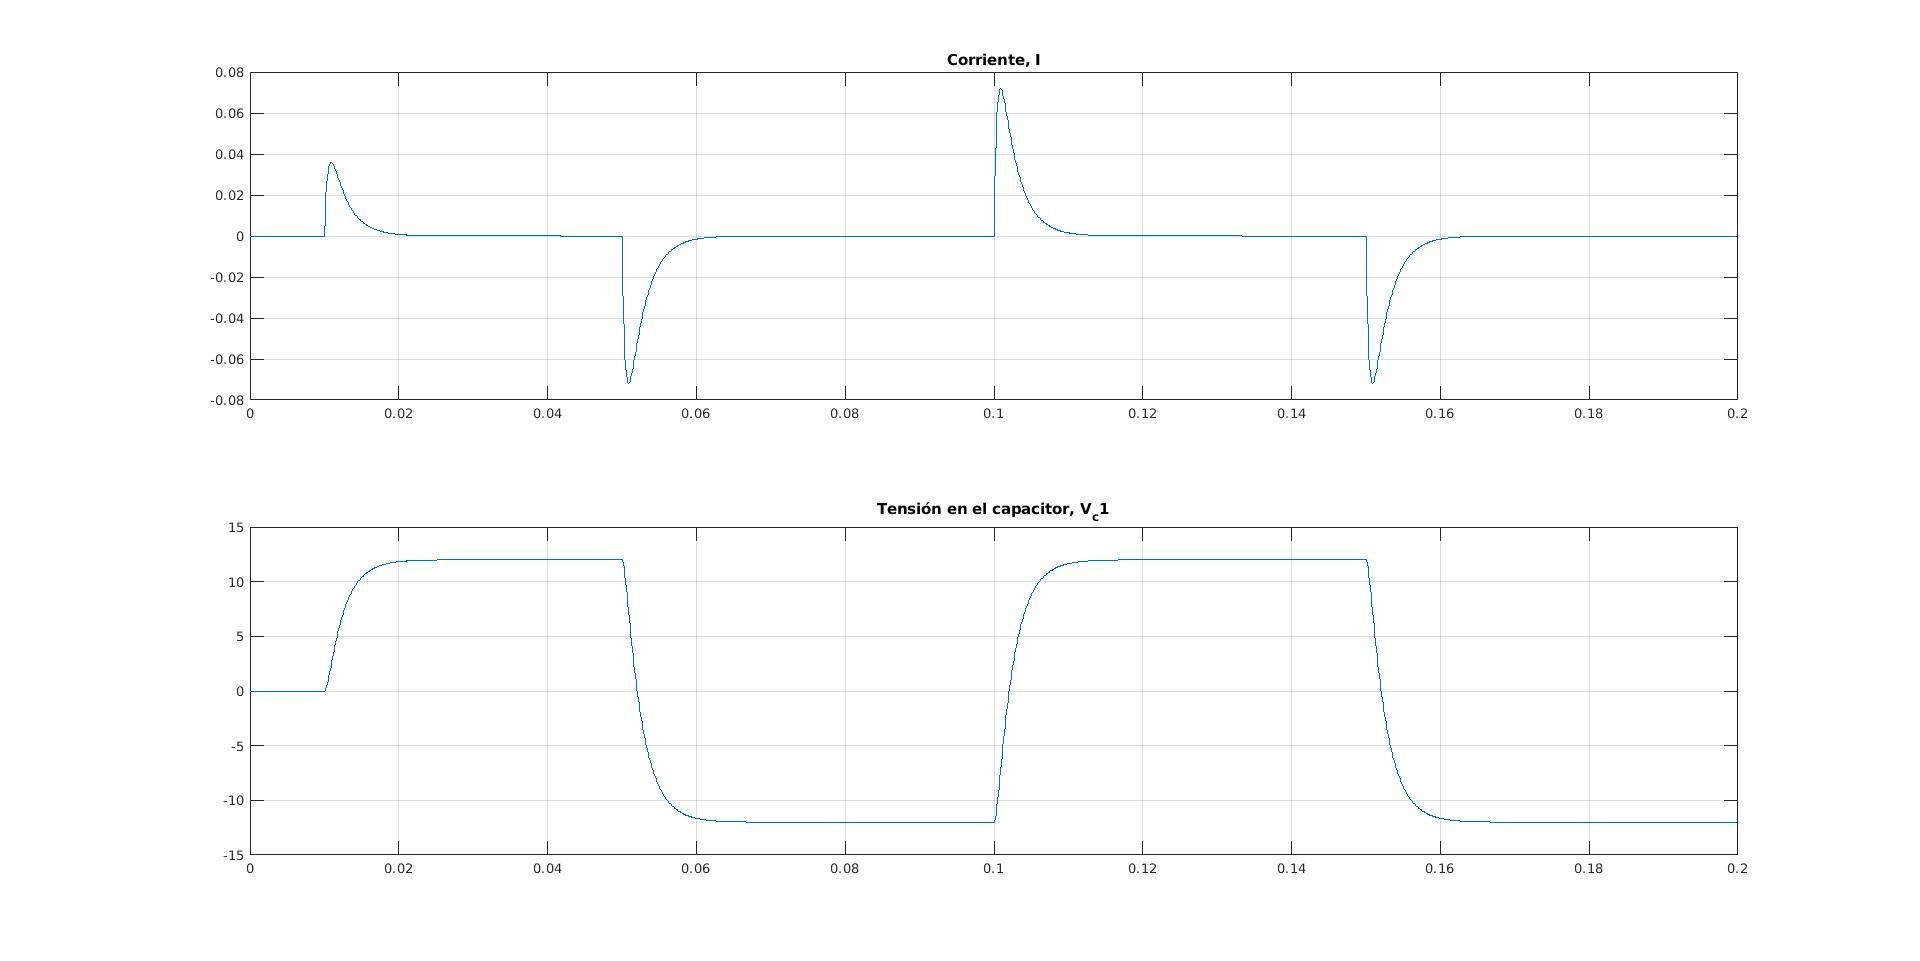
\includegraphics[width=1\textwidth]{img/rlc2-1.jpg}
  \caption{Datos medidos del circuito RLC}
\end{figure}

En condiciones iniciales nulas, al energizar el circuito el capacitor y el inductor se comportarán como 
un corto circuito durante un breve periodo hasta que finalice el transitorio. Es por esto que podemos realizar
una primera aproximación de la resistencia del circuito observando la amplitud del primer pico de corriente y la 
tensión de alimentación.

Esta primera aproximación da como resultado:

$$R_{aporx}=\frac{V_{max}}{I_max} = 335\Omega$$

Según las ecuaciones matemáticas que modelan al sistema RLC, 

$$\frac{di}{dt} = -\frac{R}{L}i - \frac{1}{L}v_c +\frac{1}{L}v_e$$

$$\frac{di}{dt} = \frac{1}{C}i$$

podemos obtener la función de transferencia del sistema

$$G(s)=\frac{I(s)}{V_e(s)}= \frac{1}{LCs^2+CRs+1}$$

Se logra observar que la función de transferencia del sistema es de segundo orden. 

Para obtener el valor de $L$ y $C$ es necesario identificar la función de transferencia del sistema medido. Se implementa
el método de Chen tomando tres puntos equidistantes que abarquen la mayor parte del transitorio.

\begin{lstlisting}[language=matlab]
  % Determinamos el modelo del circuito RLC a partir del metodo desarrollado
  % por Chen
  
  % td: tiempo entre puntos equidistantes para el algoritmo de chen
  % t1: tiempo inicial para el algoritmo
  td = 0.01;
  t1 = 0.002;
  k=max(v_c);
  [val lugar] = min(abs((t1+td)-t))
  
  k1 = v_c(lugar)/k-1
  [val lugar] = min(abs((2*t1+td)-t))
  k2 = v_c(lugar)/k-1
  [val lugar] = min(abs((3*t1+td)-t))
  k3 = v_c(lugar)/k-1
  
  b=4*k1^3*k3-3*k1^2*k2^2-4*k2^3+k3^2+6*k1*k2*k3;
  alfa1 = (k1*k2+k3-sqrt(b))/(2*(k1^2+k2));
  alfa2 = (k1*k2+k3+sqrt(b))/(2*(k1^2+k2));
  beta= (2*k1^3+3*k1*k2+k3-sqrt(b))/sqrt(b);
  
  T1 =-t1/log(alfa1);
  T2 =-t1/log(alfa2);
  %T3 = beta*(T1-T2)+T1
  
  s = tf('s');
  
  %sys_id = k*(T3*s+1)/(T1*s+1)/(T2*s+1)
  sys_id = k/(T1*s+1)/(T2*s+1)
  \end{lstlisting}

  La función de transferencia del sistema identificado es:
   
  $$G_{id}(s) = \frac{1}{\num{9.865e-07}s^2+\num{2.69e-3}+1}$$



  \begin{figure}[!h]
    \centering
    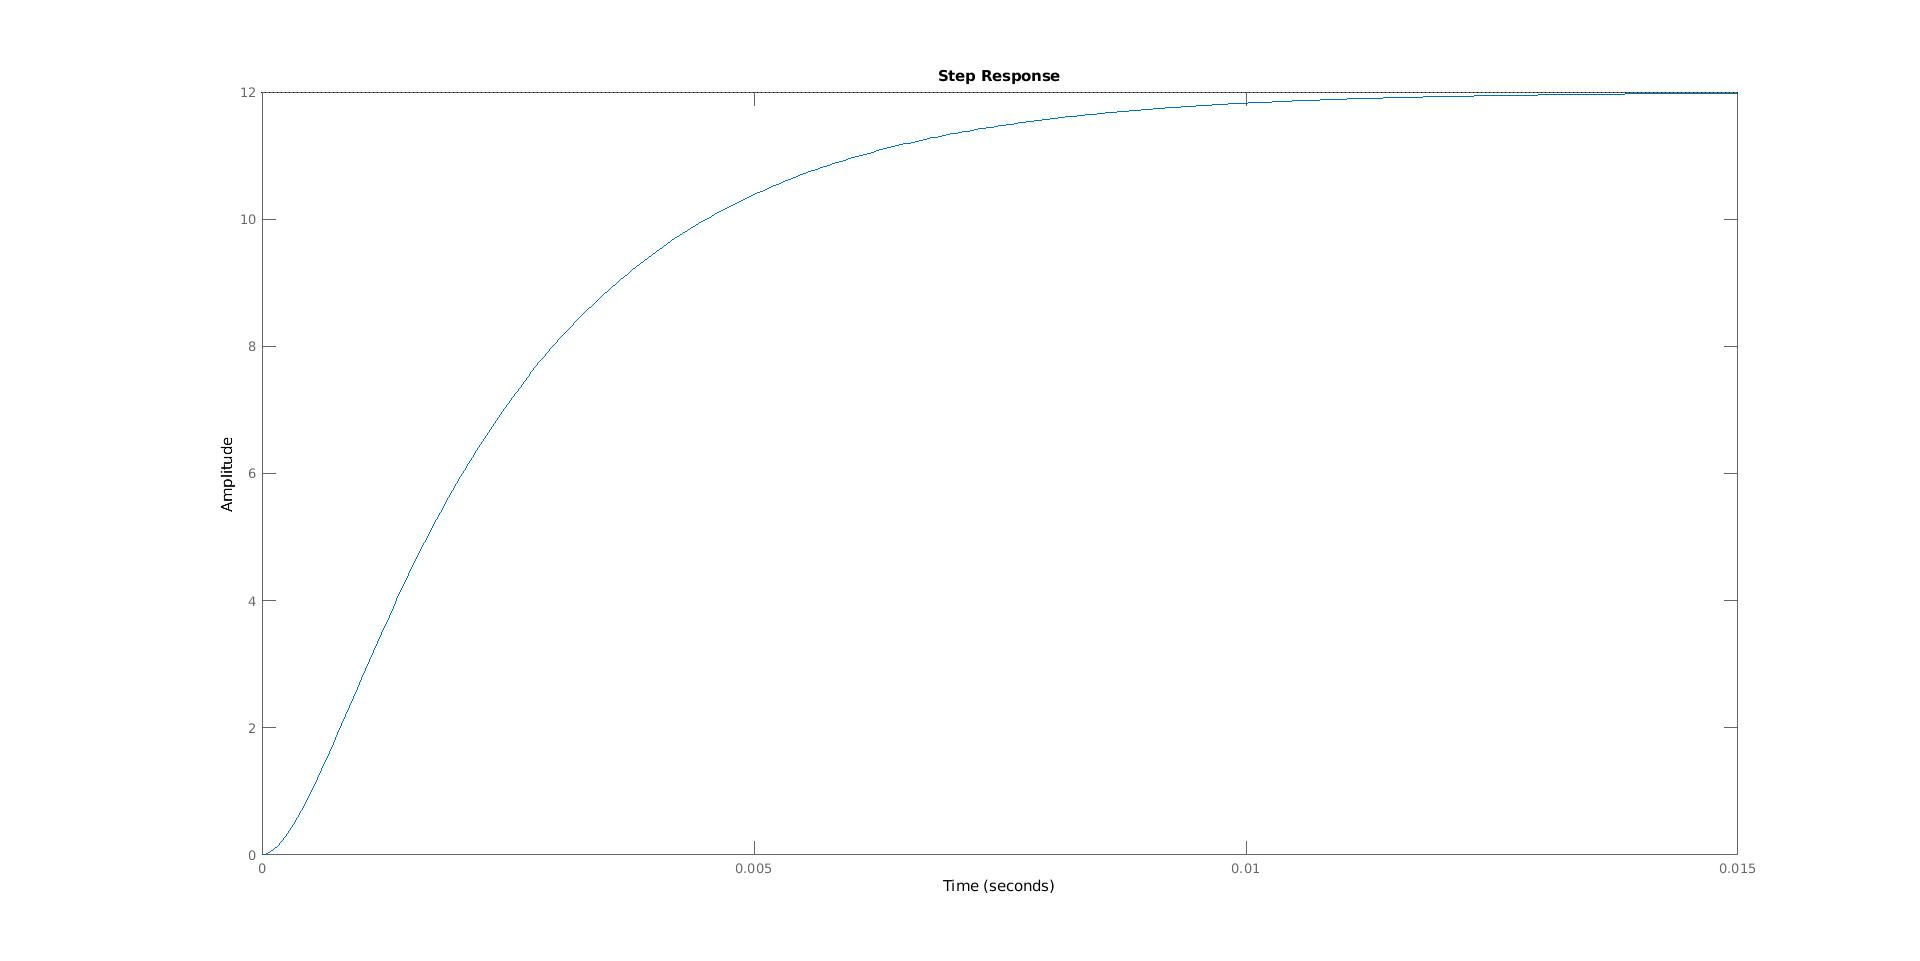
\includegraphics[width=1\textwidth]{img/rlc2-2.jpg}
    \caption{Respuesta al escalón del sistema identificado}

  \end{figure}

  A partir de la respuesta al impulso, podemos suponer que posee dos polos reales y distintos y 
  ningún cero, por lo que al realizar el algoritmo de Chen es posible descartar el cero compuesto por $T_3$.

  Al comparar la función de transferencia del sistema identificado y la obtenida de las ecuaciones matemáticas
  que lo modelan, se puede despejar los valores restantes.

  \begin{lstlisting}[language=matlab]    
[N D] = tfdata(sys_id, 'v')

C = D(2)/R
L = D(1)/C
  \end{lstlisting}

  Obteniendo los valores de $R=335\Omega$, $L=122.9mHy$ y $C=8.03\mu F$
  \par
  \textbf{Ítem (3)} Una vez determinados los parámetros R, L y C, emplear la serie de corriente desde
  0.05seg en adelante para validar el resultado superponiendo las gráficas.

  A partir del modelo de variables de estados realizamos una simulación utilizando \textit{lsim}.

  \begin{lstlisting}[language=matlab]    
[u,t] = gensig("square",0.08,0.16,0.00005);
u = -(24*u-12);
A4 = [-R/L -1/L; 1/C 0];
B4 = [1/L; 0];
C4 = [1, 0];
D4 = [0];

% Creamos modelo de espacio de estados
sys_est = ss(A4,B4,C4,D4);

[i_est,t_sim]=lsim(sys_est,u,t);
 
figure('Name','1.3')
hold on
plot(t, i_est)
plot(datos(:,1)-0.01,datos(:,2));grid on; title('Corriente');
legend('RLC estimado','RLC medido')
xlim([0 0.08])
      \end{lstlisting}

      \begin{figure}[!h]
        \centering
        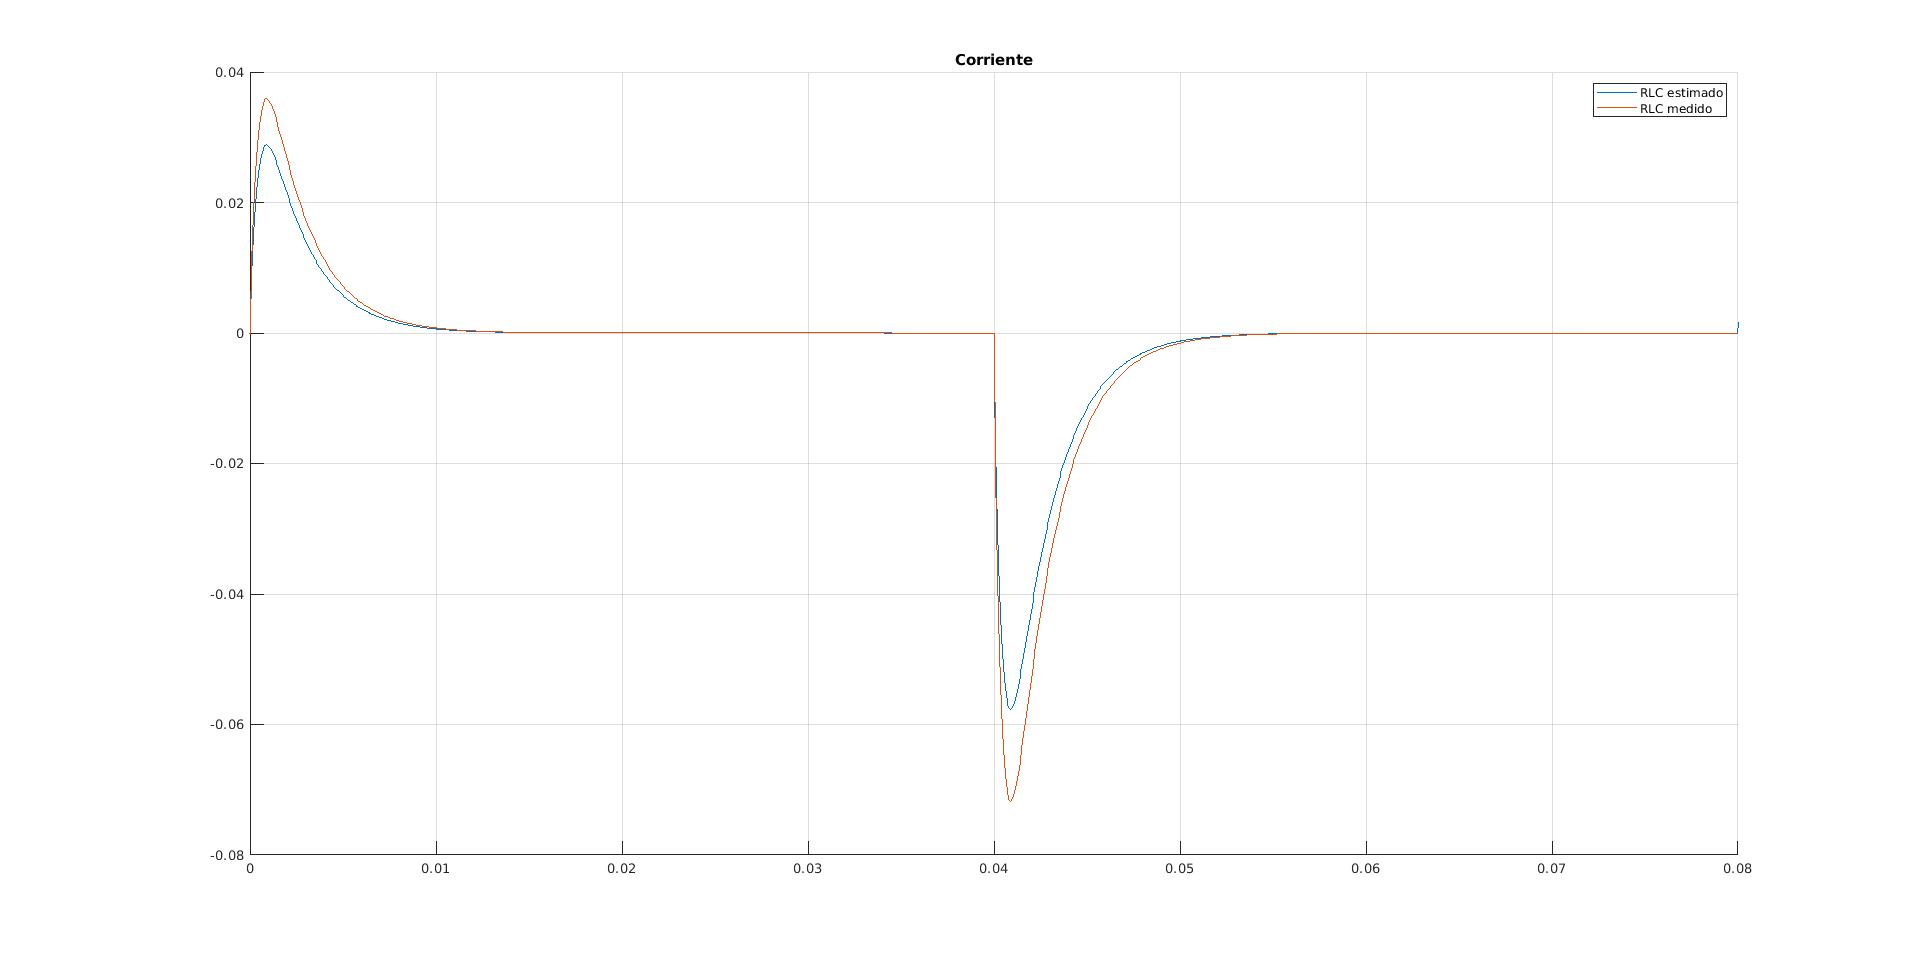
\includegraphics[width=1\textwidth]{img/rlc3-1.jpg}
        \caption{Sistema identificado vs sistema medido}
      \end{figure}

  A partir de estos resultados se puede iterar sobre el valor de R para llegar a una aproximación mas
  correcta del valor de la misma. Si modificamos $R = 270\Omega$ y volvemos a calcular los parámetros según el procedimiento
  anterior, obtenemos:

  $$R=270\Omega$$
  $$L=99mHy $$
  $$C=9.96\mu F$$

  \begin{figure}[!h]
    \centering
    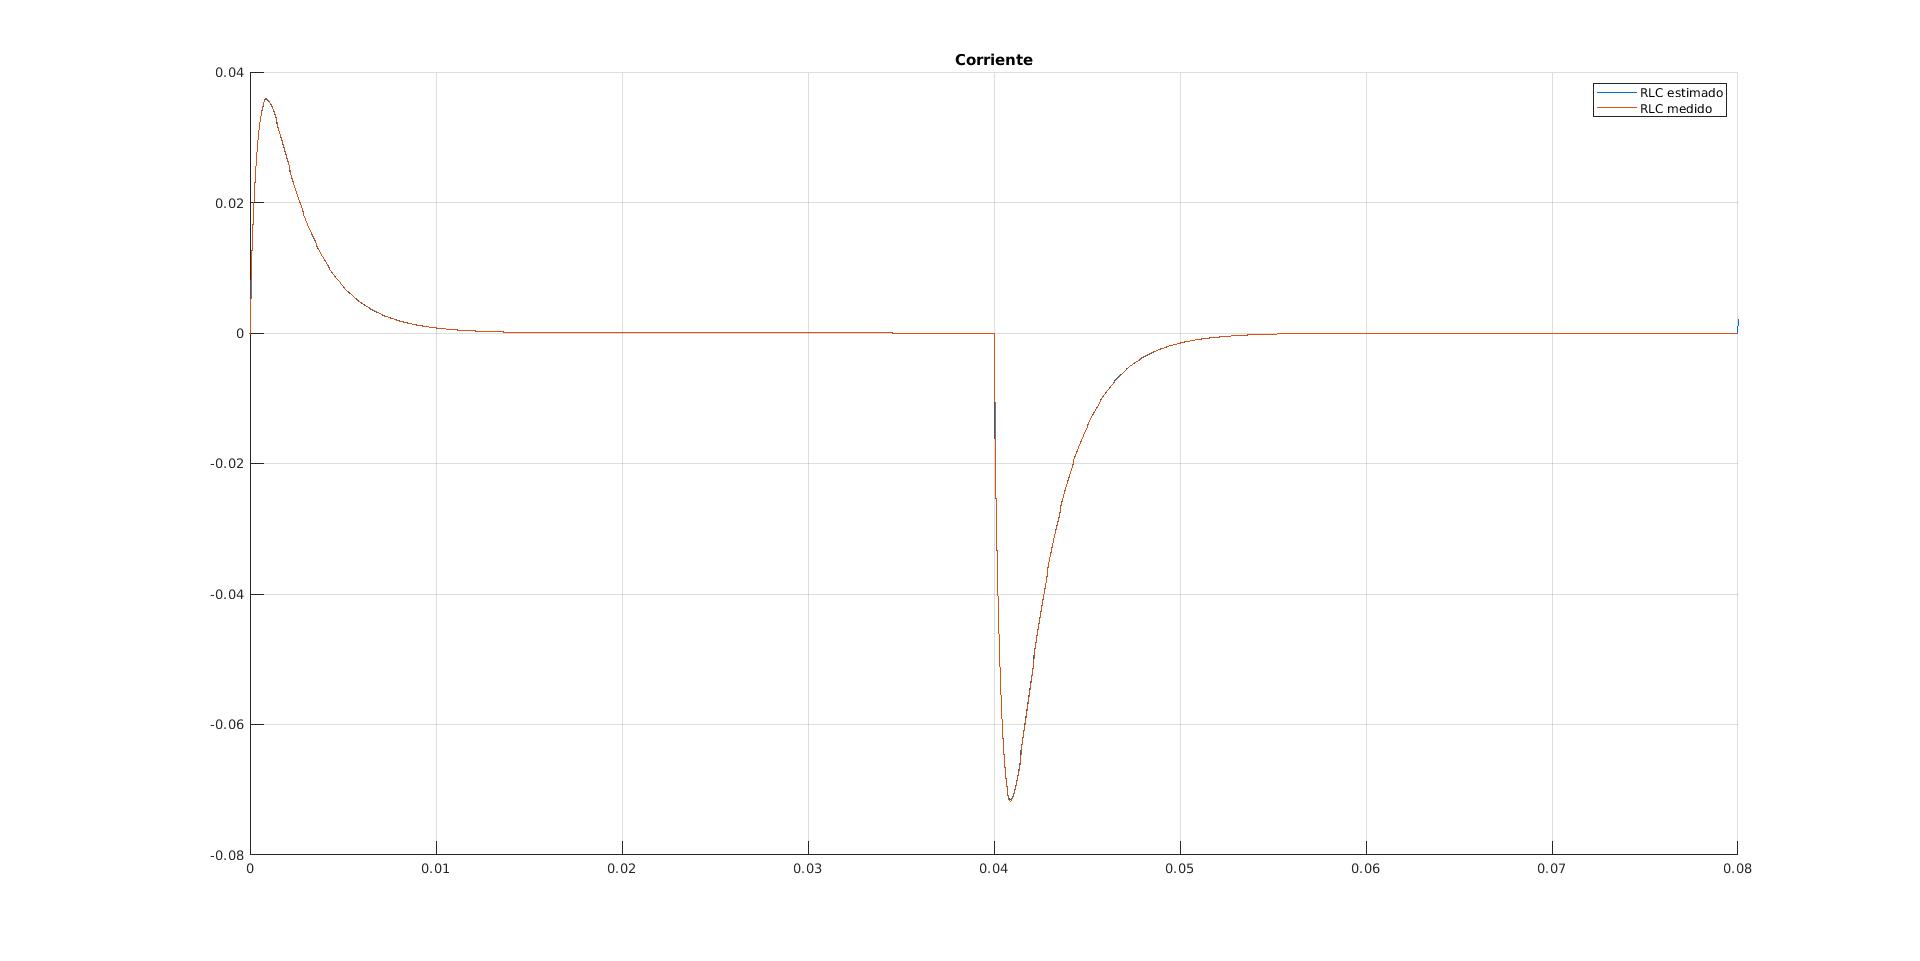
\includegraphics[width=1\textwidth]{img/rlc3-2.jpg}
    \caption{Sistema identificado vs sistema medido, con una mejor aproximación}
  \end{figure}

  Obteniendo una mejor aproximación, como se muestra en la Figura 6.

  \newpage
  \subsection{Caso de estudio 2. Sistema de tres variables de estado}
  \label{subsection:2}
  Dadas las ecuaciones del motor de corriente continua con torque de carga $T_L$ no nulo, con los parámetros $L_{AA}=\num{366e-6};J_{m}=\num{5e-9};R_A=55,6;B=0;K_i=\num{6.49e-3};K_m=\num{6.53e-3}$
  
  $$\frac{di_a}{dt} = -\frac{R_A}{L_{AA}}i_a - \frac{K_m}{L_{AA}}\omega_r +\frac{1}{L_{AA}}v_a$$

  $$\frac{d\omega_r}{dt} = \frac{K_i}{J}i_a - \frac{B_m}{J}\omega_r -\frac{1}{J}T_L$$

  $$\frac{d\Theta_t}{dt} = \omega_r$$
  
  Implementar un algoritmo de simulación para inferir el comportamiento de las variables interés
mediante integración Euler con $t_s=\num{1e-7}$ segundos para calcular su operación con un controlador

\textbf{Ítem (4)} Obtener el torque máximo que puede soportar el motor modelado mediante las ecuaciones
diferenciales cuando se lo alimenta con 12V, graficando para 5 segundos de tiempo la velocidad
angular y corriente $i_a$ para establecer su valor máximo como para dimensionar dispositivos
electrónicos.

Se realiza una simulación mediante Euler para estudiar la corriente pico de consumo del motor.

\begin{lstlisting}[language=matlab]    
%Asignamos los valores correspondientes al motor
clear all;
close all;
Laa=366e-6;
J=5e-9;
Ra=55.6;
B=0;
Ki=6.49e-3;
Km=6.53e-3;
delta=10e-07;
ts=5;
 
%Generamos la funcion de entrada de tension Va y TL para el motor.
 
Va=12;
t=0:delta:(ts-delta);
T_L = t>=0;
for i=1:ts/delta-delta
T_L(i)=0;
end

%Realizamos la integracion por euler
ia = zeros(1,ts/delta);
wr = zeros(1,ts/delta);
o = zeros(1,ts/delta);
ia(1)=0; wr(1)=0; o(1)=0; %Cond. iniciales
Va=12;

for i=2:(ts/delta-1)
 ia(i)=ia(i-1)+delta*(-Ra*ia(i-1)/Laa-Km*wr(i-1)/Laa+Va/Laa);
 wr(i)=wr(i-1)+delta*(Ki/J*ia(i-1)-B/J*wr(i-1)-T_L(i-1)/J);
 o(i) = o(i-1) + delta*wr(i-1);
end

figure('Name','Torque vs Corriente')
 subplot(2,1,1);plot(t,wr);grid on; title('Velocidad angular, W_r'); 
 subplot(2,1,2);plot(t,ia);grid on; title('Corriente de armadura, I_a');
\end{lstlisting}
  
\begin{figure}[!h]
  \centering
  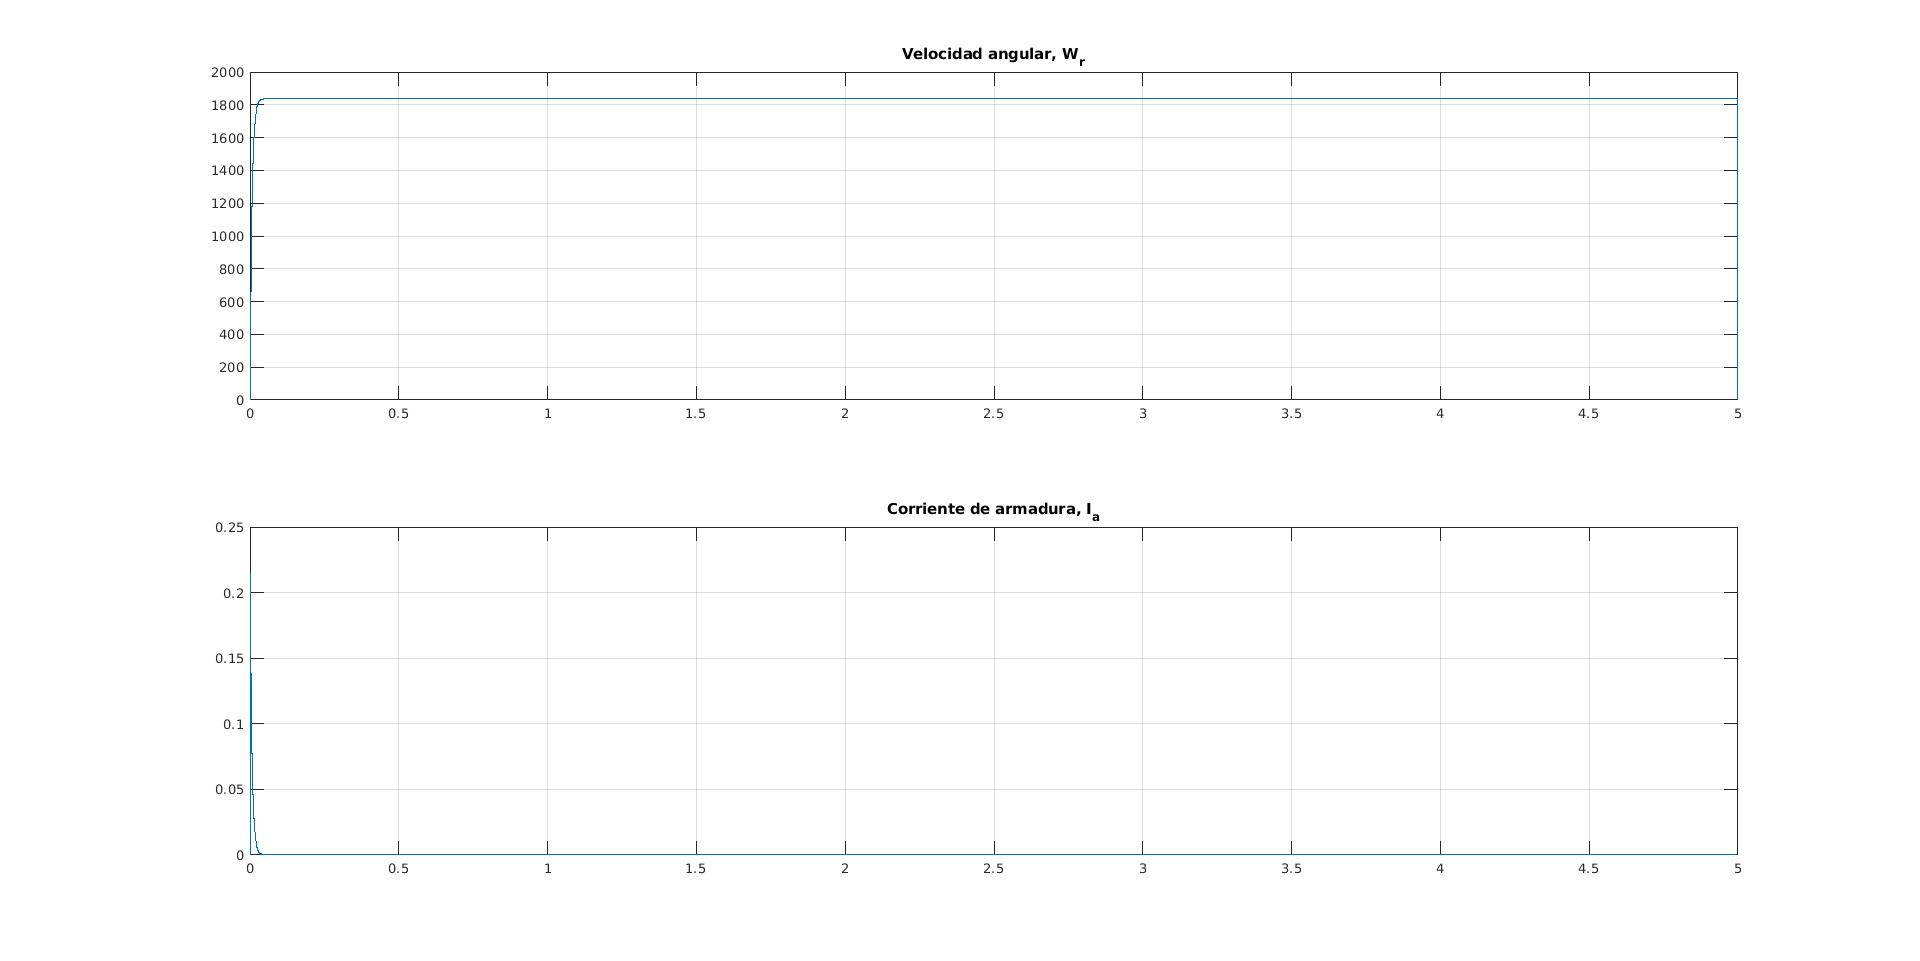
\includegraphics[width=1\textwidth]{img/mot4-1.jpg}
  \caption{Simulación del motor CC}
\end{figure}

El consumo máximo de corriente del motor, así como el torque máximo
que este nos produce, viene dado por el pico producido en el arranque.

\begin{lstlisting}
ia_max = max(ia)
wr_max = max(wr)
T_L_max = Ki*ia_max-B*wr_max
\end{lstlisting}

$$i_{a,max}=0.2147 A$$
$$T_{L,max}=0.0014 Nm$$

Se puede comprobar que este es el torque máximo si se lo aplica al modelo.

\begin{lstlisting}
%Se comprueba que son los valores maximos al aplicar un torque equivalente en
%el modelo y observar que la velocidad angular se reduzca a cero.

T_L = t>=0;
for i=1:ts/delta/2
    T_L(i)=0;
end
T_L = T_L*0.0014;
ia(1)=0; wr(1)=0; o(1)=0; %Cond. iniciales
Va=12;
for i=2:(ts/delta-1)
    ia(i)=ia(i-1)+delta*(-Ra*ia(i-1)/Laa-Km*wr(i-1)/Laa+Va/Laa);
    wr(i)=wr(i-1)+delta*(Ki/J*ia(i-1)-B/J*wr(i-1)-T_L(i-1)/J);
    o(i) = o(i-1) + delta*wr(i-1);
end

figure('Name', 'W_r al aplicar T_L maximo')
plot(t, wr)
  
\end{lstlisting}

\begin{figure}[!h]
  \centering
  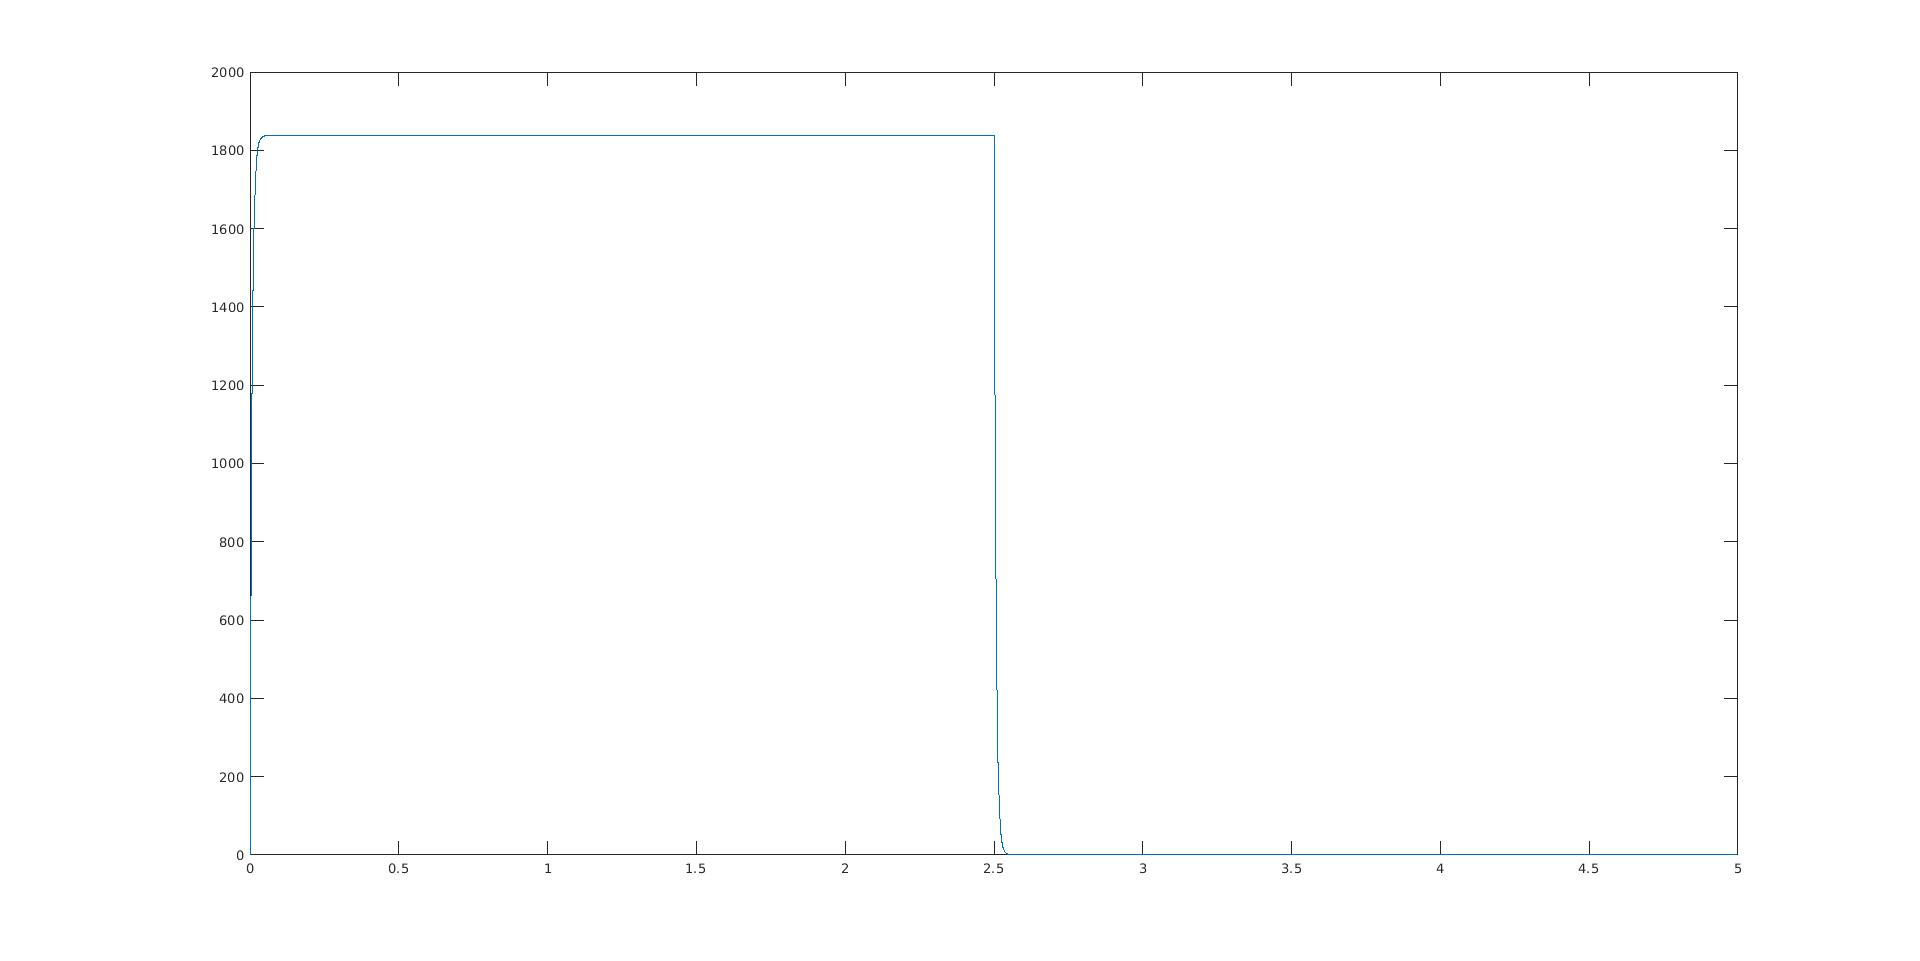
\includegraphics[width=1\textwidth]{img/mot4-2.jpg}
  \caption{Velocidad angular al aplicar el torque máximo luego de los 2.5 segundos}
\end{figure}

\textbf{Ítem (5)} A partir de las curvas de mediciones de las variables graficadas, se requiere
obtener el modelo del sistema considerando como entrada un escalón de 12V, como salida a la
velocidad angular, y al torque de carga TL aplicado una perturbación. En el archivo
\textit{Curvas\_Medidas\_Motor.xls} están las mediciones, en la primer hoja los valores y en la segunda
los nombres. Se requiere obtener el modelo dinámico, para establecer las constantes del modelo

\begin{lstlisting}[language=matlab]
% Cargamos los datos medidos
datos = xlsread('Curvas_Medidas_Motor_2024.xlsx');
t = datos(:,1);
w_r= datos(:,2);
i_a = datos(:,3);
u = datos(:,4);
t_l = datos(:,5);

figure('Name', 'Item 5')
subplot(4,1,1);plot(t,i_a);grid on; title('Corriente de Armadura, i_a');
subplot(4,1,2);plot(t,w_r);grid on; title('Velocidad Angular, W_r');
subplot(4,1,3);plot(t,u);grid on; title('Tension de entrada, V_i');
subplot(4,1,4);plot(t,t_l);grid on; title('Torque de carga, T_L');
\end{lstlisting}

\begin{figure}[!h]
  \centering
  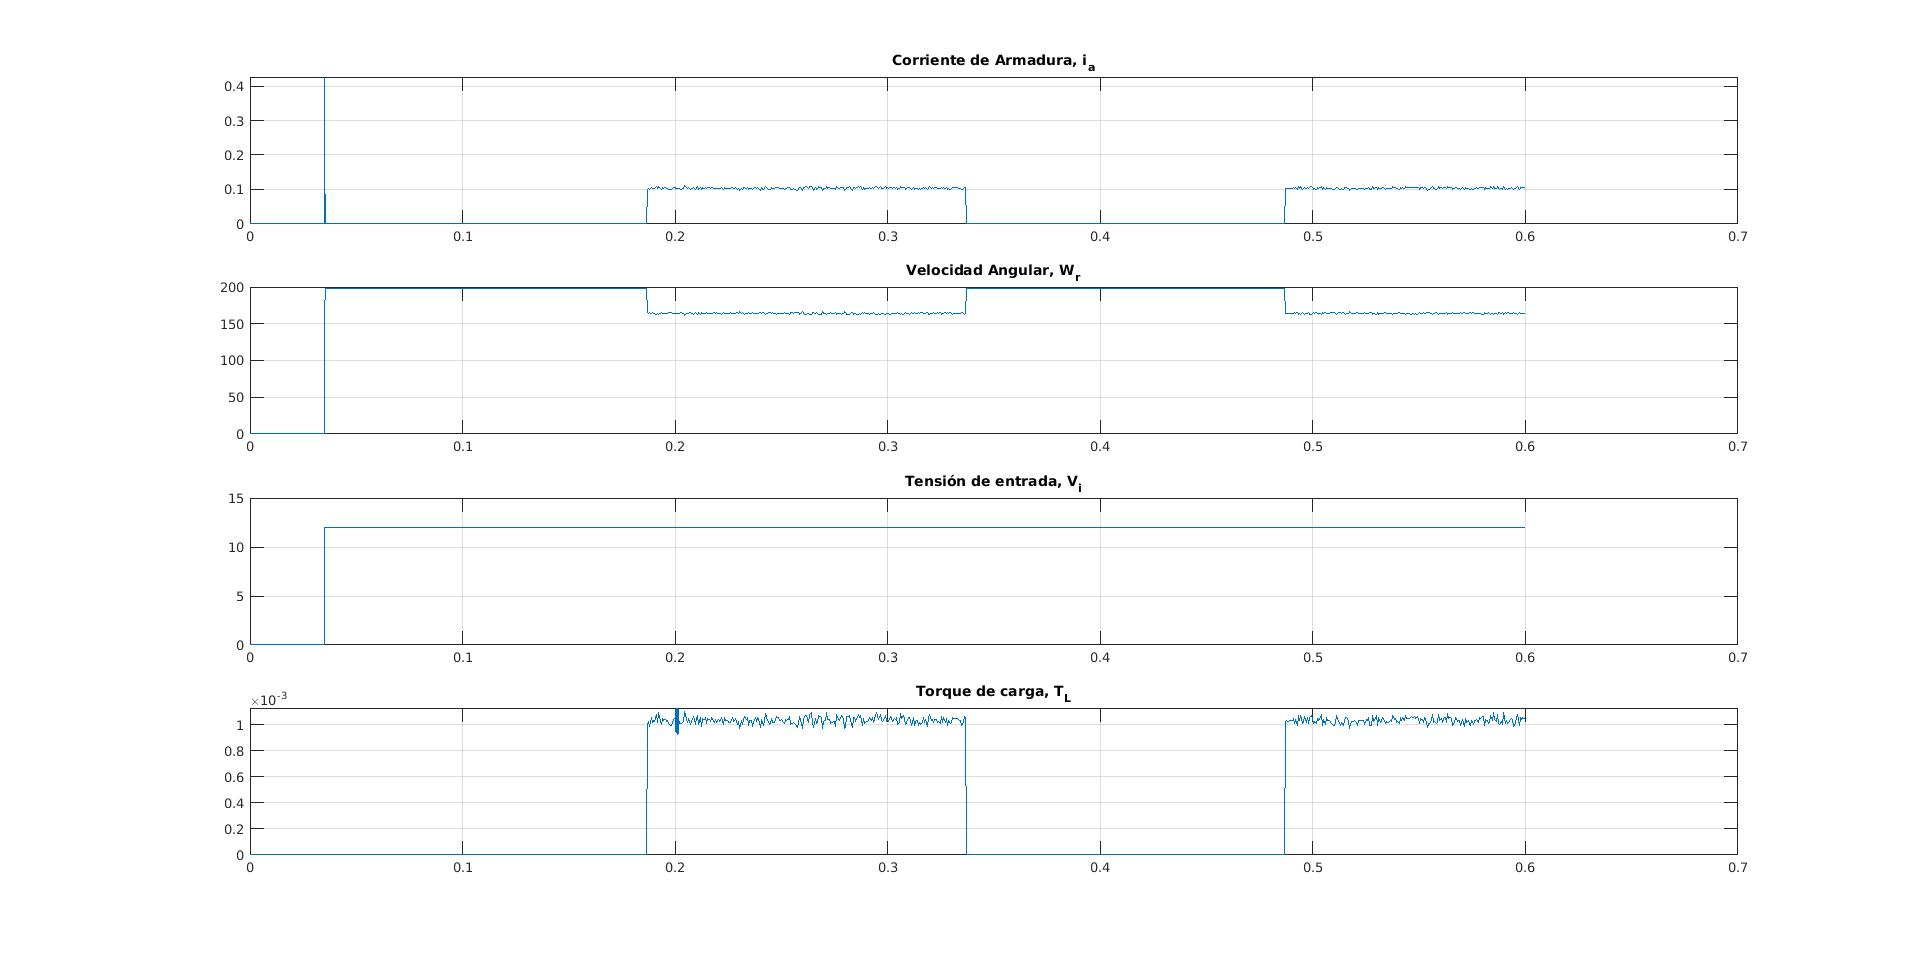
\includegraphics[width=1\textwidth]{img/mot5-1.jpg}
  \caption{$I_a, \omega_r, V_i, T_L$ medidos}
\end{figure}

Para identificar el modelo, primero se obtiene la función de 
transferencia matemática del motor, a partir de sus ecuaciones diferenciales.

Puesto que $B_m$ es chico, podemos aproximarlo a 0 para la obtención de los parámetros.

\begin{lstlisting}[language=matlab]
%% Obtencion de la funcion de transferencia del motor
syms V Ra La I Ki w Jm Km Bm Tl s real
eq1=s*I==-Ra/La*I-Km/La*w+1/La*V;
eq2=s*w==Ki/Jm*I-Bm/Jm*w;
S1=solve(eq1,eq2,w,V);
wr_va=collect(S1.w/S1.V,s);


syms V Ra La I Ki w Jm Km Bm Tl s real
eq1=s*I==-Ra/La*I-Km/La*w;
eq2=s*w==Ki/Jm*I-Bm/Jm*w-Tl/Jm;
S1=solve(eq1,eq2,w,Tl);
wr_tl=collect(S1.w/S1.Tl,s);


% tomamos Bm = 0
wr_va = subs(wr_va, Bm, 0)
wr_tl = subs(wr_tl, Bm, 0)
pretty(wr_va);
pretty(wr_tl);  
\end{lstlisting}

Las funciones de transferencia que modelan al motor, tomando como salida solamente
la velocidad angular $\omega_r$ son

$$\frac{W_r(s)}{V_a(s)}=\frac{K_i}{J_mL_{AA}s^2+J_m R_as+K_iK_m}$$
$$\frac{W_r(s)}{T_L(s)}=\frac{-R_a-L_{AA}s}{J_mL_{AA}s^2+J_m R_as+K_iK_m}$$

La ganancia en estado estable de las funciones se puede obtener
mediante el teorema del valor final para las mismas. Tomamos los siguientes limites

\[ \lim_{s\to0} \frac{s}{s}\frac{W_r(s)}{V_a(s)} = \frac{1}{K_m}\]
\[ \lim_{s\to0} \frac{s}{s}\frac{W_r(s)}{T_L(s)} = \frac{-R_a}{K_iK_m}\]

\begin{lstlisting}[language=matlab]
% Segun TVF tenemos
limit(wr_va, s, 0)
limit(wr_tl, s, 0)  
\end{lstlisting}

A partir de los datos medidos, se puede aproximar $R_a$ con un método similar al usado para el circuito RLC.
Puesto que en el arranque, con condiciones iniciales nulas, el bobinado del motor se comporta como un circuito casi resistivo, la aproximación
$$R_a = V_a/I_{a,max}$$
es válida. Por lo tanto, 

\begin{lstlisting}[language=matlab]
Ra = max(u)/max(i_a)  
\end{lstlisting}

$$R_a = 28.13\Omega$$

A su vez, el valor de la velocidad angular $\omega_r$ en estado estacionario está determinado
por la constante del motor $K_m$ para la función de transferencia $\frac{W_r(s)}{V_a(s)}$, por
lo que podemos calcular $K_m$ a partir del valor de $\omega_r$ para un torque de carga nulo $T_L = 0$.

\begin{lstlisting}[language=matlab]
Km = max(u)/max(w_r)
\end{lstlisting}

$$K_m = \num{60.5e-3}$$

Al aplicar el torque $T_L$, $\omega_r$ cae de $198rad/s$ a $164rad/s$. Por linealidad, se puede inferir que esto es producto
de sumar el aporte de la función de transferencia $\frac{W_r(s)}{T_L(s)}$, que relaciona la velocidad con el torque. Entonces, la ganancia
en estado estacionario de $\frac{W_r(s)}{T_L(s)}$ tiene signo negativo y se puede calcular a partir de los 
parámetros obtenidos anteriormente. Debido a que la velocidad disminuye, la ganancia tendrá signo negativo y su valor es

$$K_{ss} = \frac{-(192-164)}{\num{1.05e-3}} = \num{3.23e4}$$

con la cual es posible despejar

$$K_i = \frac{R_a}{K_mK_{ss}} =\num{14.4e-3}$$

Usando el algoritmo de Chen se logra identificar la función de transferencia $\frac{W_r(s)}{V_a(s)}$

\begin{lstlisting}[language=matlab]
%% Determinamos las funciones de transferencia a partir del metodo desarollado
% por Chen

% td: tiempo de delay de entrada
% t1: tiempo inicial para el algoritmo

td = 0.0351;
t1 = 0.0001;
%k=max(w_r);
k = 198
[val lugar] = min(abs((t1+td)-t))

k1 = w_r(lugar)/k-1;
[val lugar] = min(abs((2*t1+td)-t));
k2 = w_r(lugar)/k-1;
[val lugar] = min(abs((3*t1+td)-t));
k3 = w_r(lugar)/k-1;
%k1 = 135.58/k-1
%k2 = 191.60/k-1
%k3 = 198.30/k-1

b=4*k1^3*k3-3*k1^2*k2^2-4*k2^3+k3^2+6*k1*k2*k3;
alfa1 = (k1*k2+k3-sqrt(b))/(2*(k1^2+k2));
alfa2 = (k1*k2+k3+sqrt(b))/(2*(k1^2+k2));
beta= (2*k1^3+3*k1*k2+k3-sqrt(b))/sqrt(b);

T1 =-t1/log(alfa1);
T2 =-t1/log(alfa2);
%T3 = beta*(T1-T2)+T1
s = tf('s');
G1=(k)/(T1*s +1)/(T2*s +1); %G1 normalizada.
G1=G1/12;

figure
hold on
step(G1*12,5e-4, 'r') %Simulo aplicando 12V a la entrada.
plot(datos(:,1)-0.0351,datos(:,2));grid on; title('Velocidad Angular W_r');
legend('FdT estimado','FdT medido')
hold off
\end{lstlisting}

\begin{figure}[!h]
  \centering
  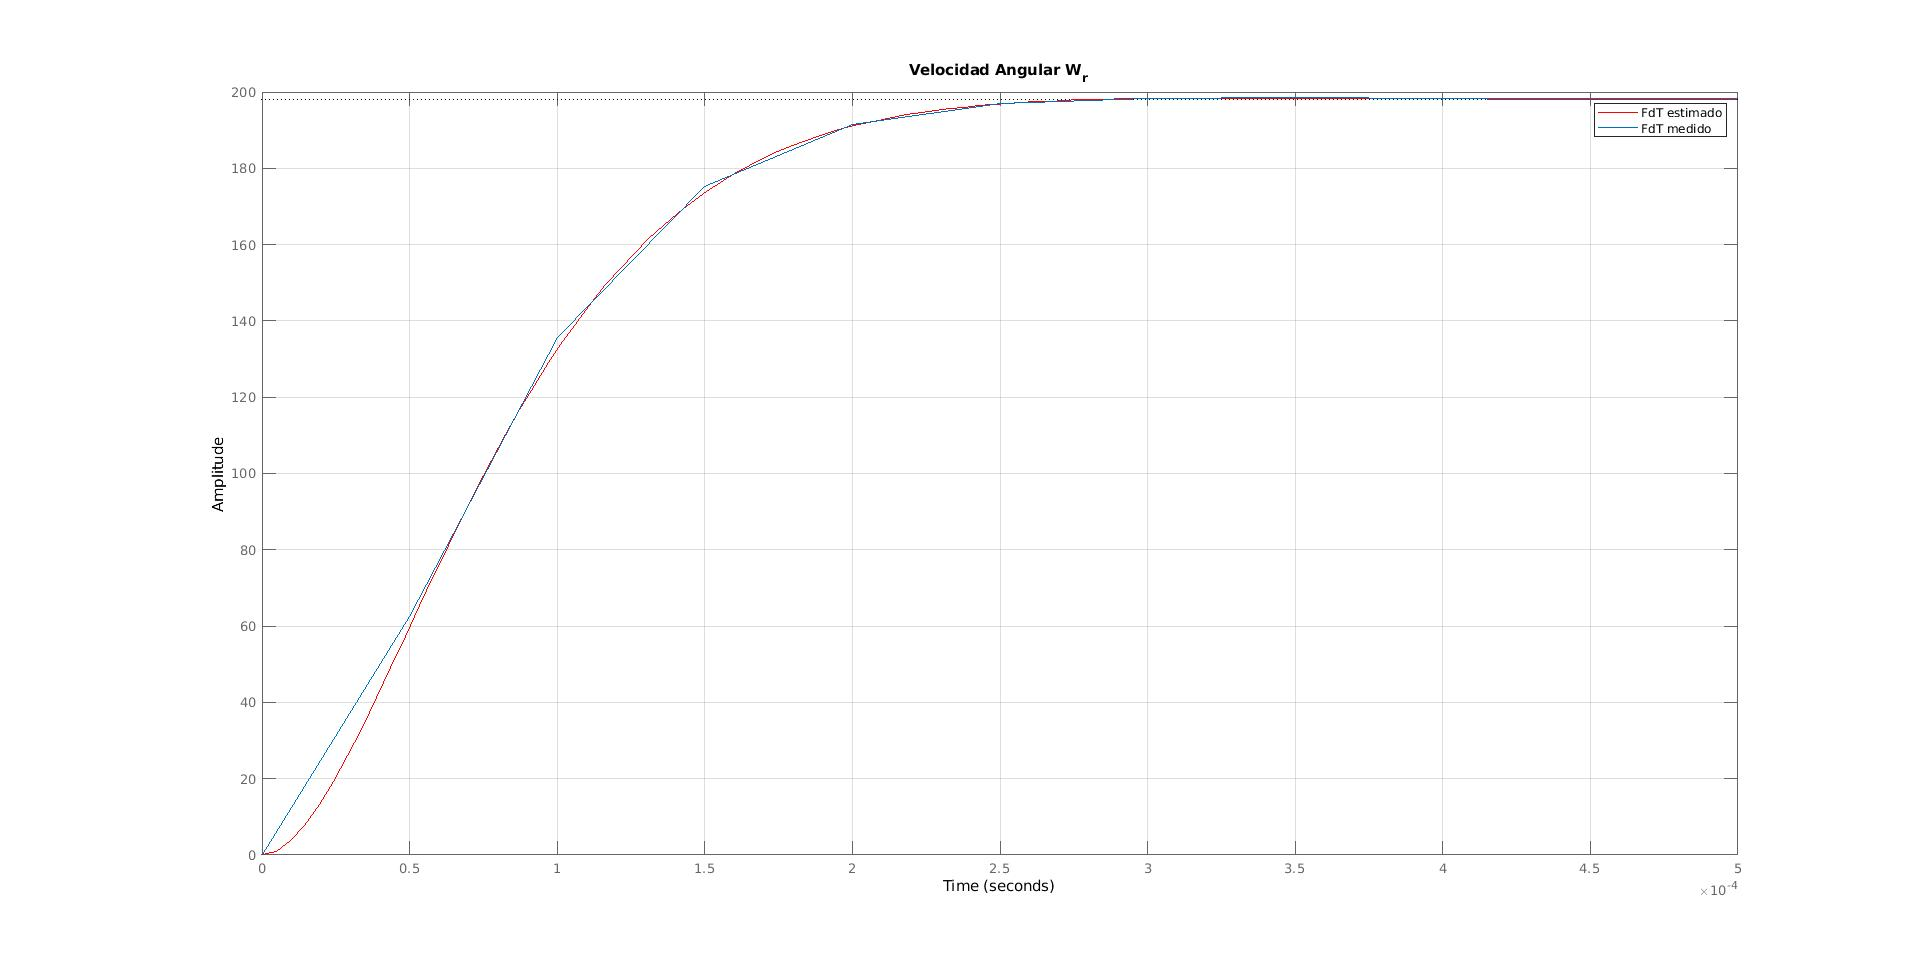
\includegraphics[width=1\textwidth]{img/mot5-2.jpg}
  \caption{$\frac{W_r(s)}{V_a(s)}$ medido vs identificado}
\end{figure}

Así, la funcion de transferencia que relaciona la velocidad angular con la identificada
es

$$\frac{W_r(s)}{V_a(s)}=\frac{16.5}{\num{2.23e-9}s^2+\num{8.43e-5}s+1}$$

Para obtener los parámetros del motor restante, se puede comparar la función de transferencia
identificada con la función obtenida mediante sus ecuaciones diferenciales, tal que

$$\frac{W_r(s)}{V_a(s)}=\frac{16.5}{\num{2.23e-9}s^2+\num{8.43e-5}s+1} = \frac{K_i}{J_mL_{AA}s^2+J_m R_as+K_iK_m}$$

Como el valor de $K_i$ es conocido, se puede multiplicar y dividir la función de transferencia identificada
para lograr que ambas estén en la misma magnitud. 

$$\frac{K_i/16.5}{K_i/16.5}\frac{16.5}{\num{2.23e-9}s^2+\num{8.43e-5}s+1} = \frac{0.0144}{\num{1.941e-12}s^2+\num{7.34e-8}s+\num{8.707e-4}} $$

Despejando las constantes,

\begin{lstlisting}[language=matlab]
[N D] = tfdata(G1, 'v')
%Normalizamos el numerador y el denominador
fac = Ki/N(3)
N = N*fac
D = D*fac

B = 0; 
J = D(2)/Ra
Laa = D(1)/J
\end{lstlisting}

obtenemos:

$$J_m = \num{2.61e-9}$$
$$L_{AA} = \num{7.43e-4}$$

Se puede comprobar si las constantes son correctas si integramos las ecuaciones diferenciales que modelan
al motor mediante Euler.

\begin{lstlisting}[language=matlab]
%Verificamos el modelo aproximado vs las mediciones
delta=1e-6;
ts=0.6;

%Generamos la funcion de entrada de tension Va y TL para el motor.
t_s =0:delta:(ts-delta);
ia = zeros(1,ts/delta);
wr = zeros(1,ts/delta);
o = zeros(1,ts/delta);
va = zeros(1,ts/delta);
T_L = zeros(1,ts/delta);
ia(1)=0; wr(1)=0; o(1)=0; %Cond. iniciales

for i=1:(ts/delta)
    if i*delta < 0.0351
        va(i) = 0;
    else
        va(i) = 12;
    end
end


 for i=1:(ts/delta)
     if i*delta < 0.1863
         T_L(i) = 0;
     elseif i*delta < 0.3372
         T_L(i) = 1.03e-3;
     elseif i*delta < 0.4866
         T_L(i) = 0;
     else
         T_L(i) = 1.03e-3;
     end
 end
        
for i=2:(ts/delta-1)
 ia(i)=ia(i-1)+delta*(-Ra*ia(i-1)/Laa-Km*wr(i-1)/Laa+va(i-1)/Laa);
 wr(i)=wr(i-1)+delta*(Ki/J*ia(i-1)-B/J*wr(i-1)-T_L(i-1)/J);
 o(i) = o(i-1) + delta*wr(i-1);
end

figure('Name','Torque vs Corriente')
 subplot(3,1,1);
 plot(t_s,wr);grid on; title('Velocidad angular, W_r'); 
 hold on
 plot(t,w_r);
 legend('Aprox', 'Medido')
 hold off
 
 subplot(3,1,2);plot(t_s,ia);grid on; title('Corriente de armadura, I_a');
 hold on
 plot(t,i_a);
 hold off
 
 
 subplot(3,1,3);plot(t_s,T_L);grid on; title('Torque de carga, T_L');
 hold on
 plot(t,t_l);
 hold off
\end{lstlisting}

\begin{figure}[!h]
  \centering
  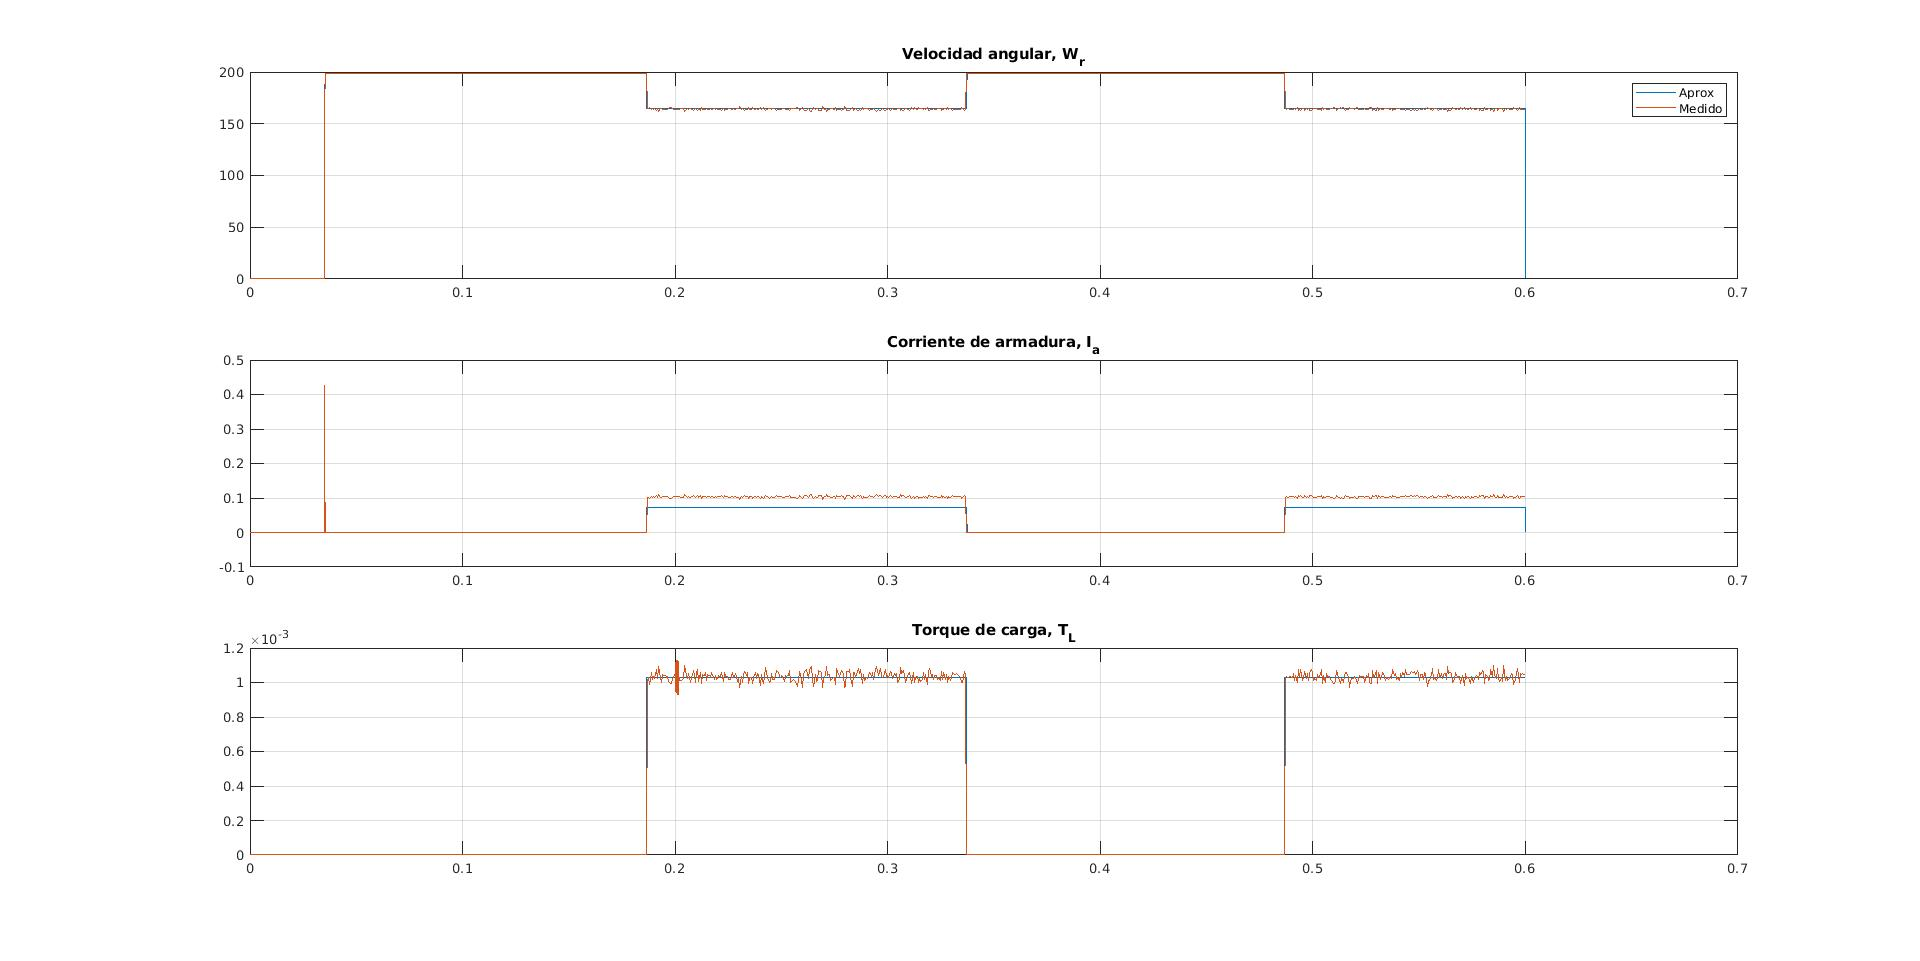
\includegraphics[width=1\textwidth]{img/mot5-3.jpg}
  \caption{Modelo medido vs modelo aproximado}
\end{figure}

Notar que existe un error en estado estacionario en la corriente de armadura $i_a$. Esto es
provocado por la forma en que se calculo $R_a$ (es solo una aproximación, no es exacto). 

\begin{figure}[!h]
  \centering
  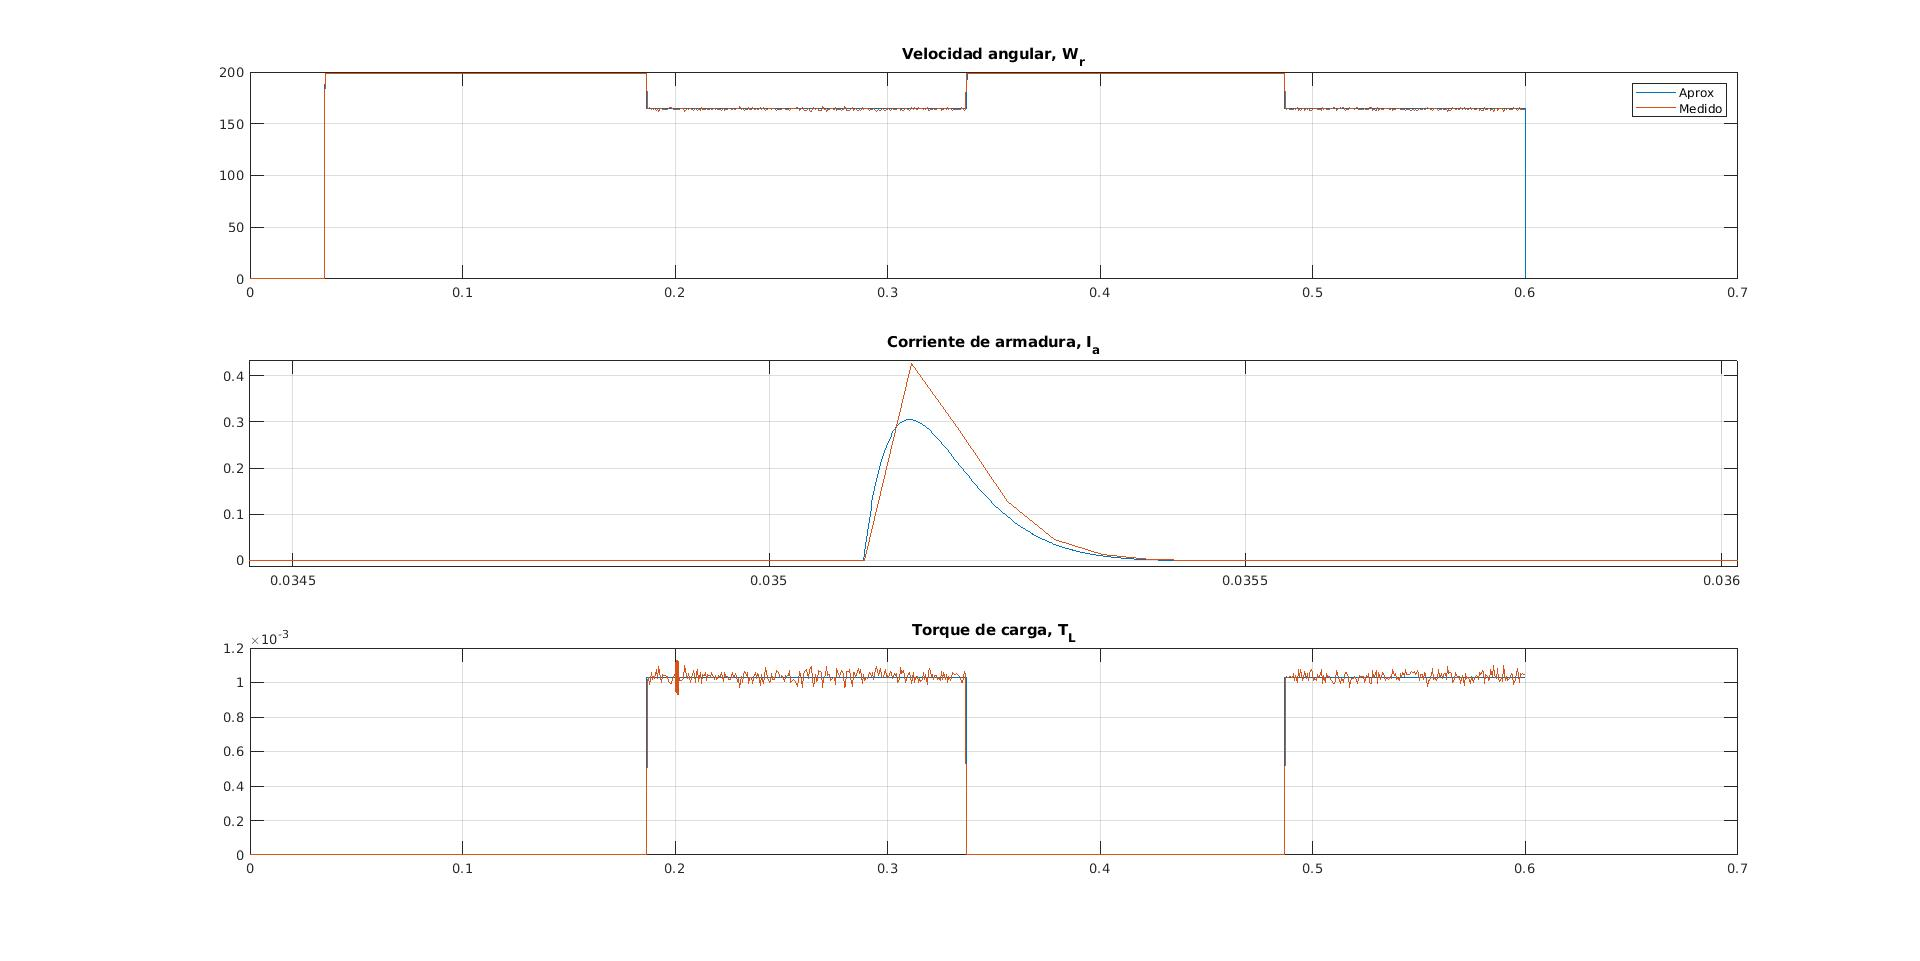
\includegraphics[width=1\textwidth]{img/mot5-4.jpg}
  \caption{El pico en la corriente en el arranque no coincide de manera exacta debido al valor incorrecto de $R_a$}
\end{figure}

Si modificamos el valor de $R_a$ de forma iterativa, para aproximar mejor el primer pico, obtenemos

$$R_a = 20\Omega$$

Debido a que $R_a$ cambió, debemos volver a calcular el valor de las constantes. Realizando el procedimiento de calculo
nuevamente obtenemos las constantes finales del motor:

$$R_a = 20\Omega$$
$$K_m = \num{60.5e-3}$$
$$K_i = \num{10.2e-3}$$
$$B = \num{0}$$
$$J_m = \num{2.61e-4}$$
$$L_{AA} = \num{5.28e-4}$$

Al simular nuevamente con los valores nuevos notamos que el error en estado estable de la corriente de armadura desapareció, según
la figura 13.

\begin{figure}[!h]
  \centering
  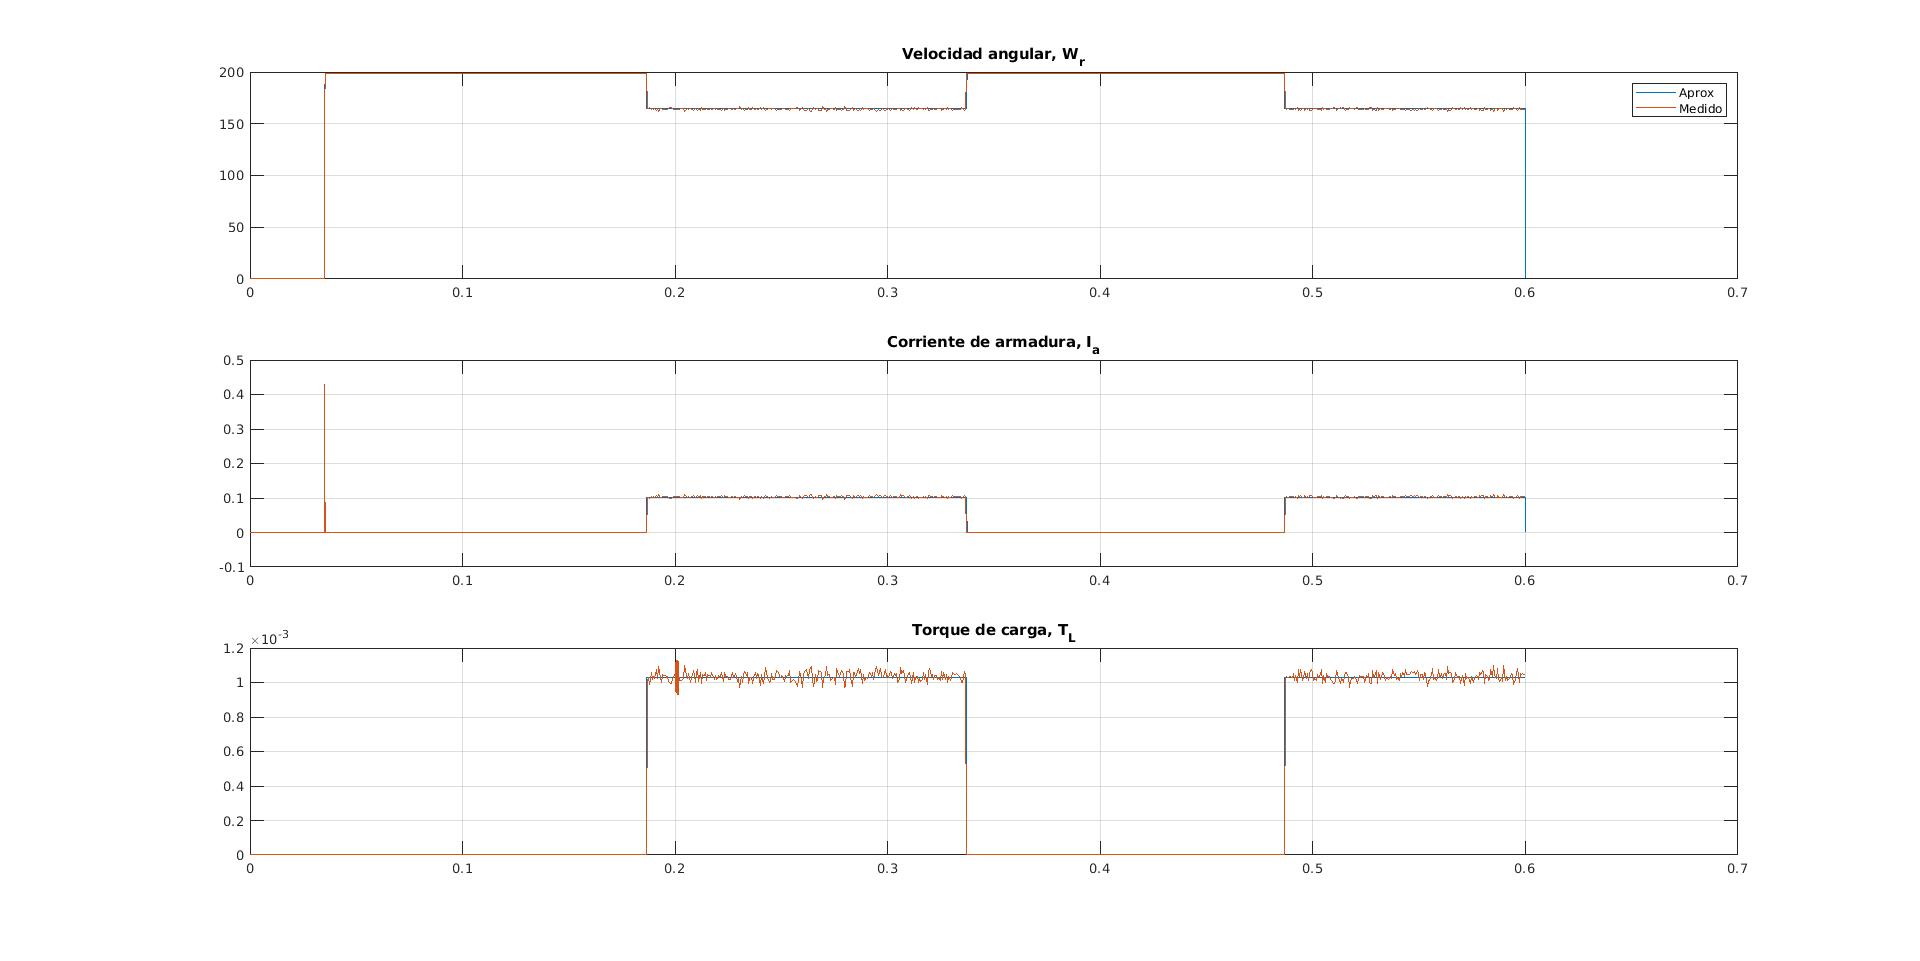
\includegraphics[width=1\textwidth]{img/mot5-5.jpg}
  \caption{Modelo medido vs modelo aproximado con el valor de $R_a$ correcto}
\end{figure}

\textbf{Ítem (6)} Implementar un PID en tiempo discreto para que el ángulo del motor permanezca en una
referencia de 1radian sometido al torque descrito en la entrada.

A partir de las ecuaciones diferenciales que modelan el comportamiento del motor, obtenemos su modelo en espacio
de estados con las siguientes matrices

\begin{center}
\begin{math}
  A = 
  \begin{bmatrix}
    -R_a/L_{AA} & -K_m/L_{AA} & 0 \\
    K_i/J_m & -B_m/J_m & 0 \\
    0 & 1 & 0
  \end{bmatrix} 
  , B =
  \begin{bmatrix}
    1/L_{AA} 0 \\
    0 -1/J_m \\
    0 0
  \end{bmatrix} 
\end{math}

\begin{math}
  C = 
  \begin{bmatrix}
    1 & 0 & 0\\
    0 & 1 & 0\\
    0 & 0 & 1
  \end{bmatrix} 
  , D = 
  \begin{bmatrix}
    0 & 0\\
    0 & 0\\
    0 & 0
  \end{bmatrix} 
\end{math}
\end{center}

A partir de las matrices de la ecuación de estado y salida, simulamos el sistema mediante Euler,
implementando un PID discreto para controlar la posición y colocando una entrada de torque
a partir de los 300ms.

Las matrices de entrada y salida son:

\begin{center}
  \begin{math}
    Y = 
    \begin{bmatrix}
      i_a\\
      \omega_r\\
      \theta_r\\
    \end{bmatrix} 
    , U =
    \begin{bmatrix}
      V_a\\
      T_L
    \end{bmatrix} 
  \end{math}
  \end{center}

Las constantes del PID se determinaron a prueba y error, resultando $K_p = 80$, $K_i=500$ y $K_d = 0.01$

\begin{lstlisting}[language=matlab]
  Laa=5.28e-04;
J=2.61e-09;
Ra=20;
B=0;
Ki=0.0102;
Km=0.0605;

A = [-Ra/Laa -Km/Laa 0; Ki/J -B/J 0; 0 1 0];
B = [1/Laa 0; 0 -1/J; 0 0];
C = [1 0 0; 0 1 0; 0 0 1];
D = [0 0; 0 0; 0 0]
U = [12; 0]

X = [0; 0; 0];
Xp = [0; 0; 0;]
ii = 0;
t_etapa = 2e-7;
tF = 600e-3;
ref = 1;

%Constantes del PID
%Kp=0.1;Ki=0.01;Kd=5;color_='r';
Kp=80;Ki=500;Kd=0.01;color_='b';
Ts=t_etapa;
A1=((2*Kp*Ts)+(Ki*(Ts^2))+(2*Kd))/(2*Ts);
B1=(-2*Kp*Ts+Ki*(Ts^2)-4*Kd)/(2*Ts);
C1=Kd/Ts;

N = tF/t_etapa
omega=zeros(1,N);
theta=zeros(1,N);
ia=zeros(1,N);
e=zeros(1,N);
acc=zeros(1,N);
ij = 0;

for ii= 1:N-1
    ij=ij+t_etapa;
    if (ij>=300e-3)
        U(2)=1e-3;
    end
    k = ii+2;
    Xp=A*X+B*U;
    X=X+Xp*t_etapa;
    Y=C*X+D*U;
    %e(k) = ref-Y(3);
    %U(1) = U(1)+A1*e(k)+B1*e(k-1)+C1*e(k-2);
    
    acc(ii+1)=U(1);
    ia(ii+1)=Y(1);
    omega(ii+1)=Y(2);
    theta(ii+1)=Y(3);
    
end

t=t_etapa:t_etapa:tF;
subplot(2,1,1);hold on;
plot(t,theta,color_);title('Salida: Posicion, \theta_t');
subplot(2,1,2);hold on;
plot(t,omega,color_);title('Salida: Velocidad, \omega_t');
xlabel('Tiempo [Seg.]');
\end{lstlisting}

\begin{figure}[!h]
  \centering
  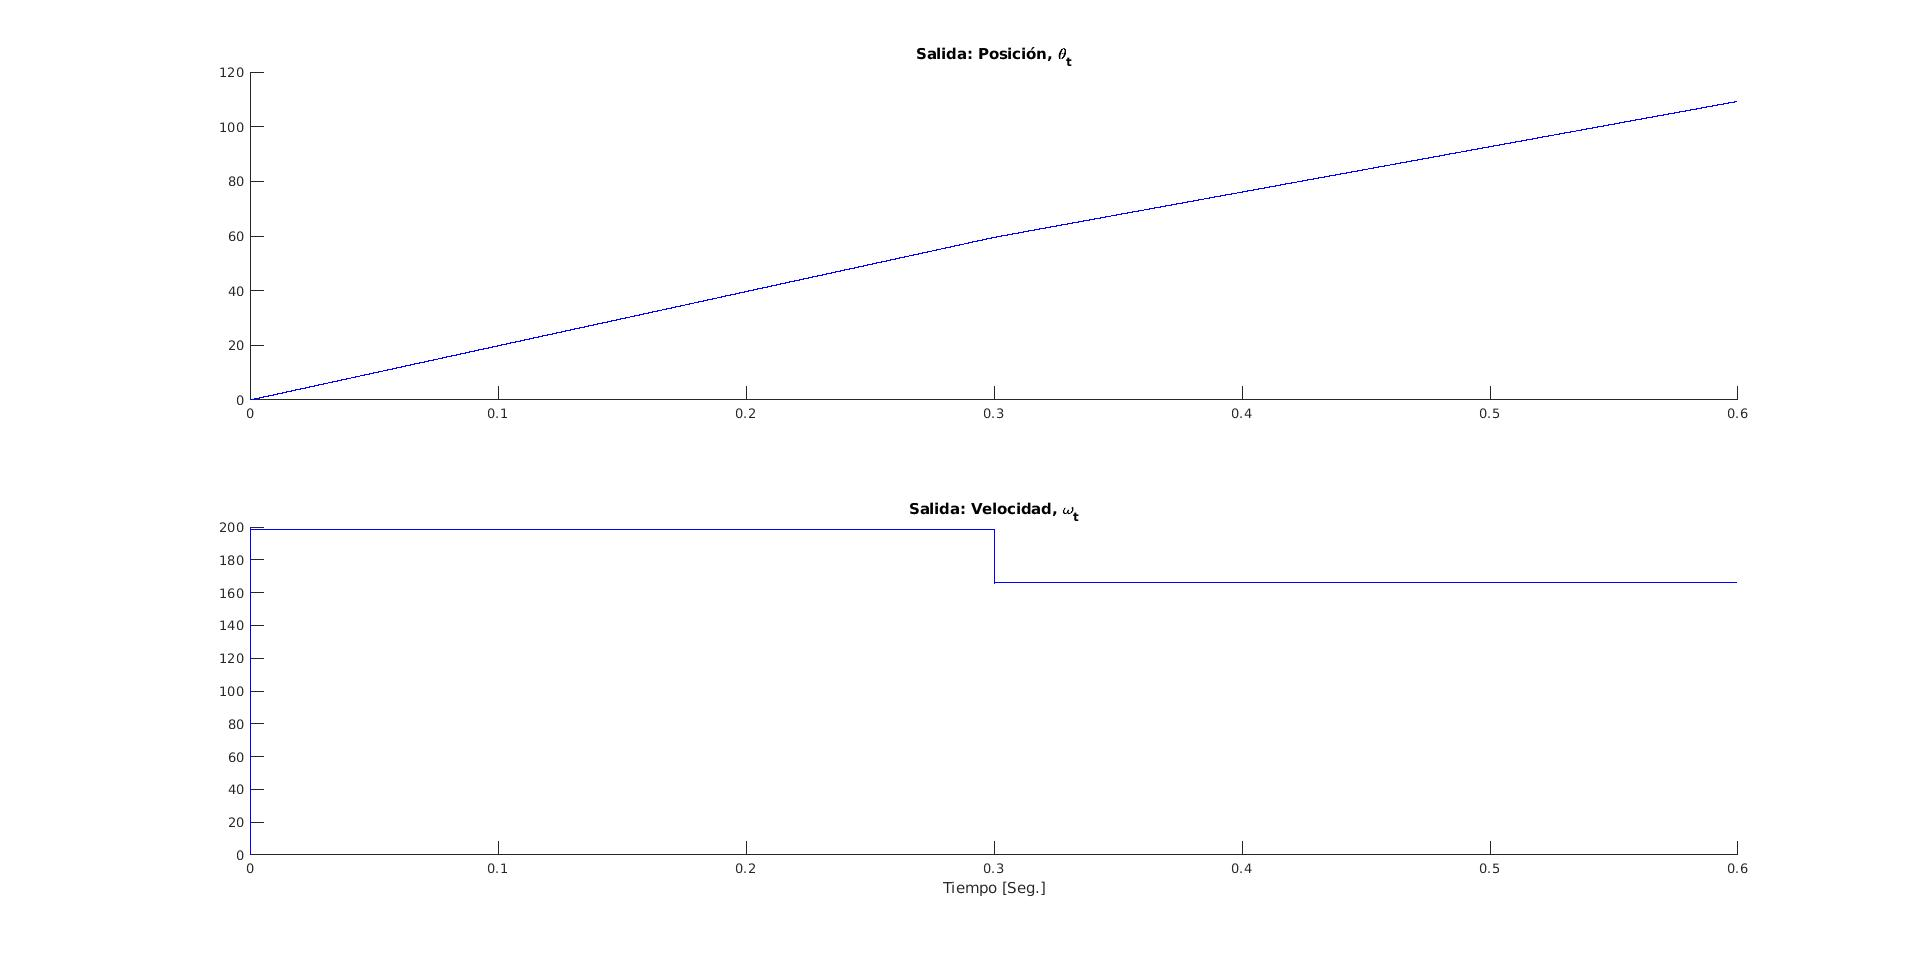
\includegraphics[width=1\textwidth]{img/mot6-2.jpg}
  \caption{Sistema sin compensar}
\end{figure}

\begin{figure}[!h]
  \centering
  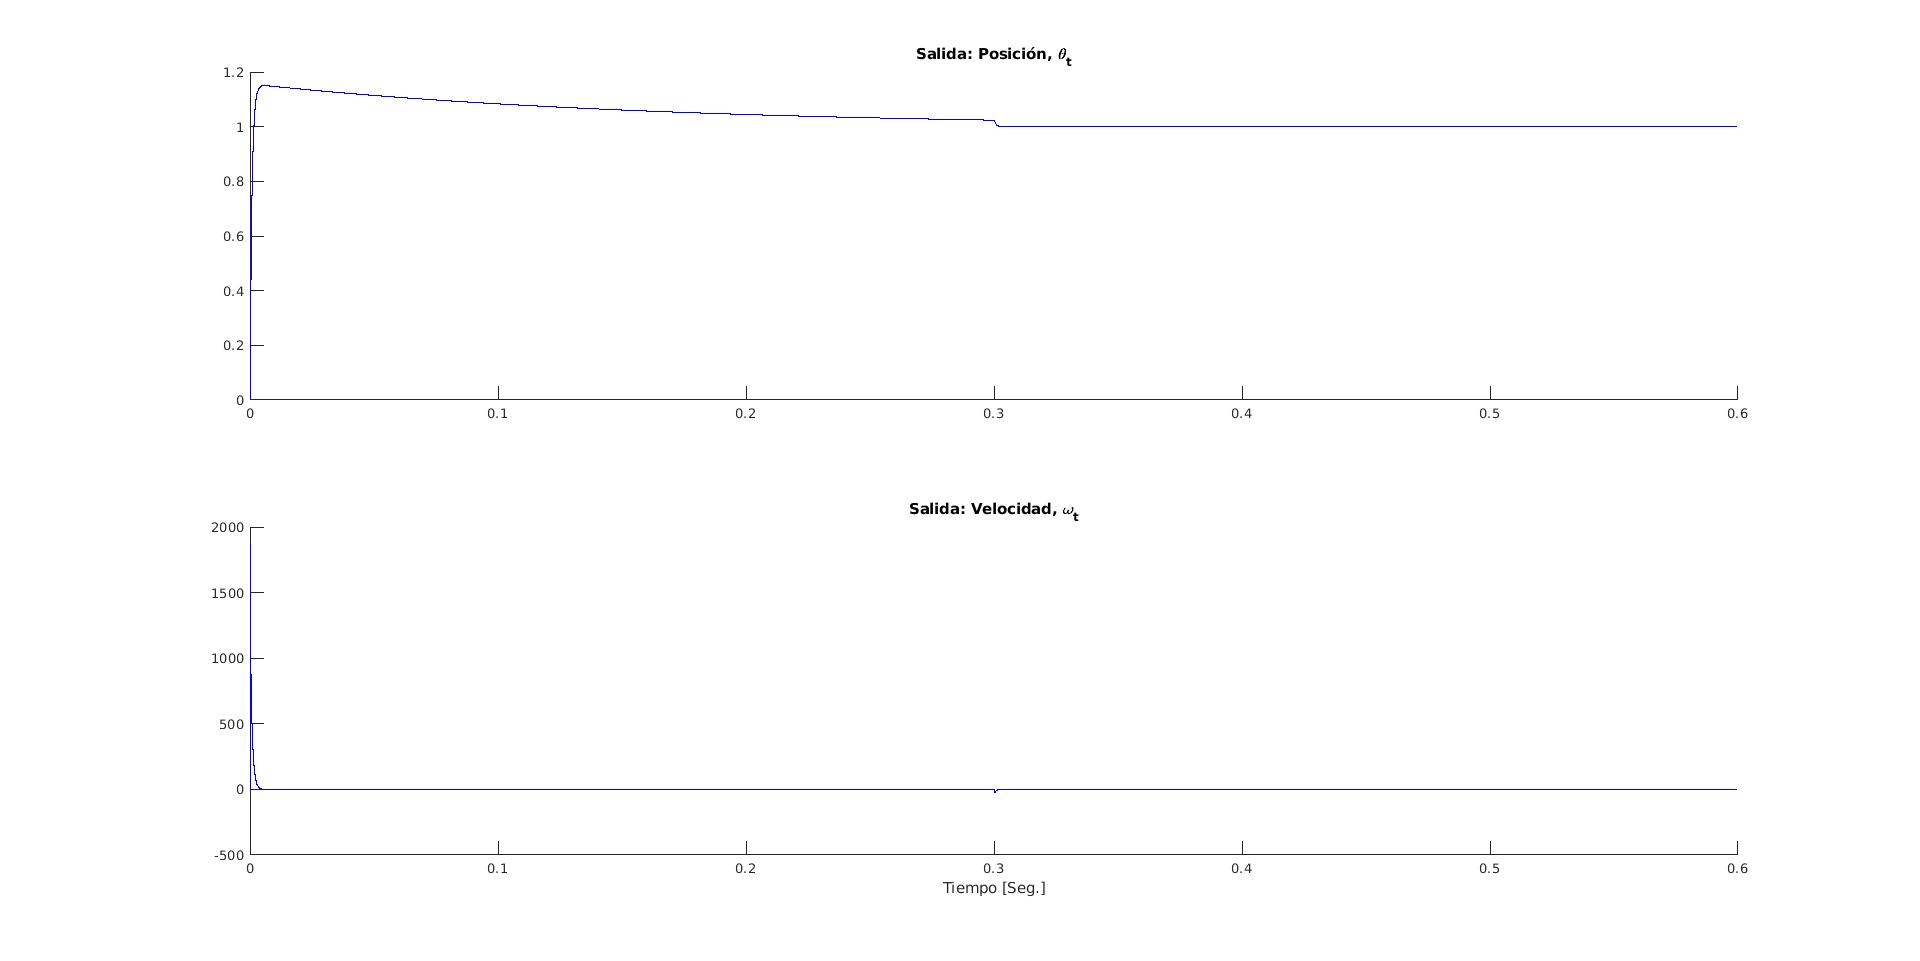
\includegraphics[width=1\textwidth]{img/mot6-1.jpg}
  \caption{Sistema compensado con PID discreto}
\end{figure}


\newpage
\section{Conclusiones}
\label{section:3}
Mediante la realización del presente trabajo, se llegaron a las siguientes
conclusiones:
\begin{itemize}
  \item Es posible y relativamente sencillo obtener las constantes que modelan de forma matemática a un sistema
  siempre y cuando sea posible medirlo.
  \item El uso de software de computo como MATLAB facilita la automatización, simulación y cálculo de procesos.
  \item El modelado en espacio de estados es una herramienta matemática sumamente útil en el análisis de 
  sistemas con varias entradas y salidas, resolviendo limitaciones que posee trabajar solamente con funciones
  de transferencia.
  \item El diseño de controladores en dominio discreto es simple y a la vez aplicable en un microcontrolador.
  \item A la hora de implementar un controlador es posible y necesario observar los parámetros eléctricos con los
  cuales el sistema interactúa. Esto ayuda a conocer los valores máximos absolutos con los cuales podemos trabajar
  para evitar la ruptura de la planta que queremos controlar. Estos valores máximos no se tuvieron en cuenta para la 
  implementación del PID discreto, lo cual podría ser un problema si se implementa sin limitar la acción de control.
  \item Se pueden relacionar de forma directa los parámetros y valores de una función de transferencia con una magnitud física.
\end{itemize}


\section{Lecciones aprendidas}
\label{section:4}
En el desarrollo del presente trabajo, se logró:
\begin{itemize}
  \item Diseñar controladores con realimentación de estados para obtener una dinámica estable considerando la dinámica y la magnitud de las acciones de control.
  \item Seleccionar las variables de estado de un proceso lineal para generar una expresión matricial lineal.
  \item Inferir la evolución temporal de procesos reales representados en variables de estado.
  \item Calcular el modelo lineal de un proceso estable multivariable a partir de su respuesta al escalón.
\end{itemize}
A su vez, es recomendable usar, dentro de lo posible MATLAB por sobre Octave. Los programas que se usaron
corrieron más rápido sobre MATLAB que sobre su alternativa open source, lo que ahorro mucho tiempo de trabajo.

También es importante destacar lo mucho que GitHub agiliza el proceso de compartir y corregir código mediante sus funciones
colaborativas.

\section{Recursos}
\label{section:5}
El código utilizado para el desarrollo del presente trabajo se encuentra en el siguiente repositorio:
\underline{\href{https://github.com/FGalvagno/sistemas-de-control}{GitHub de Facundo Galvagno}}

\end{document}

